%!TeX program = xelatex
\documentclass[12pt,hyperref,a4paper,UTF8]{ctexart}
\usepackage{CUGReport}
\usepackage{listings}
\usepackage{xcolor}
\usepackage{fontspec}
\usepackage{setspace}
\setstretch{1.5} % 设置全局行距为1.5倍
\usepackage[linesnumbered,ruled,vlined]{algorithm2e}

\usepackage{enumitem} % 载入enumitem包以便自定义列表环境
\setlist[itemize]{itemsep=0pt, parsep=0pt} % 设置itemize环境的项目间距和段落间距

\setmainfont{Times New Roman} % 英文正文为Times New Roman

%字号设置
\newcommand{\xiaochuhao}{\fontsize{36pt}{\baselineskip}\selectfont}
\newcommand{\erhao}{\fontsize{21pt}{\baselineskip}\selectfont}
\newcommand{\xiaoerhao}{\fontsize{18pt}{\baselineskip}\selectfont}
\newcommand{\sanhao}{\fontsize{15.75pt}{\baselineskip}\selectfont}
\newcommand{\sihao}{\fontsize{14pt}{18pt}\selectfont}
\newcommand{\xiaosihao}{\fontsize{12pt}{18pt}\selectfont}
%\newcommand{\wuhao}{\fontsize{10.5pt}{18pt}\selectfont}


%封面页设置
{   
	%标题
	\title{ 
		%\vspace{1cm}
		\heiti \xiaochuhao \textbf{{智能系统技术\\实践报告}} \par
		%\vspace{1cm} 
		% \heiti \Large {\underline{XXXXXX进展调研}}    
		\vspace{1cm}
	}
	
	\author{
		\vspace{0.5cm}
		\kaishu\Large 学生姓名\ \dlmu[9cm]{曾康慧} \qquad \\ %姓名 
		\vspace{0.5cm}
		\kaishu\Large 学\hspace{2em}院\ \dlmu[9cm]{未来技术学院} \qquad \\ %学院
		\vspace{0.5cm}
		\kaishu\Large 班\hspace{2em}级\ \dlmu[9cm]{220211} \\ %班级
		\vspace{0.5cm}
		\kaishu\Large 学\hspace{2em}号\ \dlmu[9cm]{20211003337} \\ %学号
		\vspace{0.5cm}
		%\vspace{0.5cm}
		\kaishu\Large 授课教师\ \dlmu[9cm]{陆承达} \qquad  \\ 
		%\vspace{1cm}
		%\vspace{0.25cm} 
	}
	\date{\today} % 默认为今天的日期,可以注释掉不显示日期
}
%%------------------------document环境开始------------------------%%
\begin{document}
	
	%%-----------------------封面--------------------%%
	\cover
	\thispagestyle{empty} % 首页不显示页码
	%%------------------摘要-------------%%
	
	\newpage
	\begin{abstract}
		
		在钻进过程中,由于钻井设备与井壁井底岩石之间等摩擦,会产生各种各样等 振动,这些振动分为:横向振动、纵向振动和扭转振动。其中扭转振动对钻井作业的危 害最大,而钻柱粘滑振动就属于扭转振动。粘滑振动是一种钻头粘滞,滑动,再粘滞,再滑动的往复性振动形式,如果不加以抑制,则会造成很严重的钻井事故,例如钻柱粘滑振动会导致钻井设备加速磨损,钻井安全性下降,钻井效率降低和钻井周期延长等不利影响。所以对钻柱粘滑振动的抑制研究非常重要。
		
		本文为抑制钻柱粘滑振动,建立了转盘、钻杆、BHA 和钻头四自由度钻柱系统扭转 模型,模型考虑了扭转自由度,钻柱阻尼和岩石钻头相互作用等高度非线性摩擦;通过 数学软件 MATLAB 和 Simulink 仿真模块对系统模型进行仿真实验,实验还原了实际钻井过程中产生等粘滑振动现象,并分析了钻井参数对粘滑振动等影响;为了抑制钻柱粘滑振动,设计了状态观测器反馈控制和PID 的控制策略,在进行控制器模型建立和参数设计后,通过仿真验证了控制策略的有效性,粘滑振动现象被消除,底部钻头转速可以稳定的跟踪顶部输入,并且能够对系统中的参数突变快速反应,使系统快速稳定。该研究结论对工程实践中钻柱粘滑振动的抑制具有重要的指导意义。
		
		
		
		\vspace{1cm}
		\textbf{关键词:} 粘滑振动; \hspace{0.5em} 扰动抑制; \hspace{0.5em} PID控制; \hspace{0.5em} 状态观测器反馈控制
	\end{abstract}
	\thispagestyle{empty} % 首页不显示页码
	
	%%--------------------------目录页------------------------%%
	\newpage
	\tableofcontents
	\thispagestyle{empty} % 目录不显示页码
	
	%%------------------------正文页从这里开始-------------------%
	\newpage
	\setcounter{page}{1} % 让页码从正文开始编号
	
	%%可选择这里也放一个标题
	%\begin{center}
	%    \title{ \Huge \textbf{{标题}}}
	%\end{center}
	
	
	
	\section{引言}
	
	
	
	\subsection{实验目的}
	对地质钻探过程和钻柱振动的基本概念有所了解;掌握 MATLAB仿真程序设计;学习钻柱系统的建模方法,设计钻柱粘滑振动主动抑制算法;利用MATLAB 进行钻柱粘滑振动分析与主动抑制仿真。
	\subsection{实习项目的研究背景}
	钻井过程是一个非常复杂的多学科交叉领域,所以在钻井过程中遇到的问题也是复杂多样的。随着钻井技术的发展,石油钻探技术在深井、超深井的开发中日渐成熟,但仍然面临着许多难题,在钻进过程中,由于钻井的深度越来越大,井下的结构也会越来越复杂,导致钻进的难度越来越大,钻井工具的振动问题也越来越剧烈。这种振动是井下钻井工具与井壁及岩石摩擦引起的振动,振动类型主要有:横向振动、轴向振动以及扭转振动三种,这三种振动类型在钻井过程中是很常见的,但是这些振动给钻井过程带来的破坏是巨大的,它们会导致钻井设备加速磨损和过早损坏、钻井安全性下降、钻井效率降低。其中扭转振动是对钻井过程造成危害最大的,扭转振动会导致钻柱系统产生粘滑振动\cite{付蒙}。
	
	粘滑振动是钻井过程中常见的一种振动形式,属于自激振荡。其表现为钻头转速某一时间段是 0-6 倍于地面转速,而另一时间段接近于 0。在钻井过程中,顶部驱动系统带动钻杆转动,钻杆带动 BHA 转动,BHA 则与钻头连接,带动钻头转动,钻头与岩石摩擦接触,当井下钻头与岩石的摩擦力矩大于顶部驱动系统给予的驱动力矩,钻头将会发生粘滞现象,即与岩石接触但不钻进,此时顶部驱动仍然给钻杆提供扭矩,扭转力矩汇集在钻杆上,可能会导致钻杆连接失效或者弯曲扭断。当顶部驱动系统提供的能量大于井下钻头与岩石之间的摩擦力矩时,钻头会摆脱粘滞状态,但由于此时驱动系统传递到钻头上的的驱动扭矩已经非常大,钻头会高速转动,从而进入滑脱状态。如此反复地进行粘滞滑脱过程,粘滑振动对钻井工具的损坏日积月累,最终造成钻井工具的不可修复、钻井安全性及钻井效率的降低。粘滑振动对钻井过程及工程人员的安全性的危害显而易见,所以钻柱系统粘滑振动的抑制消除对整个钻井过程提高钻井效率,保证钻井过程安全进行,提升我国石油资源储备量具有重大的实际意义\cite{吴永强}。
	
	传统观点认为,钻柱振动(尤其是粘滑振动)的发生与钻头-岩石作用间非线性摩擦相关,即动摩擦与静摩擦之间的相互转换。近期,有学者们逐渐认为钻头-岩石作用可能与钻头转速是无关的,钻柱振动的产生原因可能并不是单纯由于非线性摩擦效应导致。
	
	\iffalse
	\begin{itemize}
		\item \texttt{main.tex} 主文件
		\item \texttt{reference.bib} 参考文献,使用bibtex
		\item \texttt{ZJUTReport.sty} 文档格式控制,包括一些基础的设置,如页眉、标题、学院、学号、姓名等
		\item \texttt{figures} 放置图片的文件夹
	\end{itemize}
	\fi
	
	
	
	
	
	\section{钻柱粘滑振动的机理分析}
	为了抑制钻柱系统粘滑振动,首先需要了解钻柱系统产生粘滑振动现象的原因,并 且对钻柱系统的组成及工作原理进行深入了解。本章主要讲述钻柱系统的组成及其工作 原理,并对钻柱粘滑振动的发生原因进行分析。
	\subsection{钻柱系统的组成及工作原理}
	钻柱系统是钻井过程中非常重要的一部分,担负着非常重要的职责。钻柱为钻井液 提供通向钻头的通道;将地面的驱动扭矩传递给钻头,并对钻头施压,使钻头在驱动扭 矩与压力作用下进行破碎和钻入岩石;根据钻柱的长度可以大致获取该井的深度;通过 对钻柱的观察可以获取井眼、井下钻头以及底层的情况;对井下事故处理及地层压力状况进行测试与评价。它主要由井架、天车、游车、大钩、方钻杆、绞车、转盘、钻杆、 钻铤和钻头组成\cite{巩全成},如\autoref{fig:钻井系统的基本组成}。
	\begin{figure}[!htbp]
		\centering
		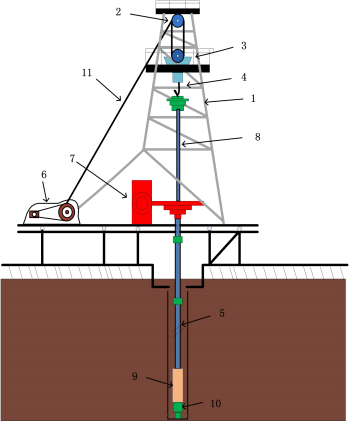
\includegraphics[width=0.5\linewidth]{figures/钻井系统的基本组成}
		\caption{钻井系统的基本组成}
		\small{1-井架,2-天车,3-游车,4-大钩,5-钻杆,6-绞车,7-转盘,8-方钻杆,9-钻铤,10-钻头,11-钢丝 绳}
		\label{fig:钻井系统的基本组成}
	\end{figure}
	
	在 \autoref{fig:钻井系统的基本组成} 中,井架是钻井或者修井时安放天车、游车、大钩和起下、存放钻杆、油 管和抽油杆的框架装置。天车和游车是组成起升系统的滑轮组。绞车通过滚筒轴上的钢丝与天车和游车连接,通过滚筒的转动并由钢丝控制起升。大钩的上部与游车连接,也是重要的起升设备。方钻杆处于钻柱的顶端,与转盘相连,用于传递转盘的扭矩和承受 钻柱的全部重量。转盘是旋转设备,通过旋转驱动钻具启动,并且通过方钻杆传递驱动 扭矩。钻杆是钻柱中最长的一段,用于传递上部旋转系统给与井下钻头的驱动扭矩、输 送钻井过程中所需的钻井液、增加钻柱长度和连接地表设备与井底设备的装置。钻铤处 于钻柱的最下部,是井下钻具组合的重要部分,主要作用是为钻头施加压力,缓解钻头处的不利振动与跳动来使钻头稳定旋转和破岩。钻头主要是用于破碎岩石和钻进的主要设备\cite{许帅}。
	
	在钻井过程中,绞车启动,通过钢丝绳带动天车游车,转盘电机驱动旋转转盘转动,旋转转盘带动方钻杆转动,方钻杆转动后带动下部钻柱和井下钻头开始转动,钻柱将从 转盘处传递下来的驱动扭矩传递到井下钻头处,并同时通过钻铤给钻头施加压力,令钻 头破碎岩石和钻进。
	
	
	\subsection{钻柱粘滑振动的机理分析}
	在石油钻井过程中,由于井深的增加,钻柱在几千米甚至上万米深的复杂环境下工作,受到的外部阻力与承受的压力是巨大的,这就需要掌握钻柱在井下的工作状态与工作能力。
	
	钻柱在起下钻时处于凌空状态,但由于重力的影响,钻柱整体处于一个拉伸的状态 下,在旋转转盘启动后,转盘带动方钻杆转动,方钻杆转动后带动钻柱开始转动,钻柱 转动后带动井下钻头旋转进行破岩,在钻进过程中,由于钻头与岩石的摩擦切削,会导 致钻井过程产生非常剧烈的振动现象,这些振动类型主要分为以下几种:横向振动、扭 转振动和轴向振动。其中横向振动是一种垂直于钻柱轴线的振动;扭转振动是钻柱在井 筒中由于井下钻头与岩石的摩擦力矩不断变化引起的弯曲振动;纵向振动是与钻柱轴线 平行的振动。钻柱振动是钻井过程中最不希望有的,长期的钻柱振动会使钻井设备受到 严重损害,使钻井作业的安全性降低,也会使钻井的效率降低。所以抑制钻柱振动,提 高钻井效率,保证钻井安全和延缓钻井设备损坏是必要的,本章主要分析由钻柱的扭转 振动产生的粘滑振动。
	
	钻柱扭转振动是引起钻柱粘滑振动的主要原因,当井底岩石与井下钻头的摩擦力矩 大于旋转转盘通过钻柱传递到钻头的驱动扭矩时,钻头会出现卡顿现象,也称为粘滞状 态,在粘滞状态时,旋转转盘一直在旋转,并且带动着方钻杆和钻柱一直转动,由于井 下钻头一直处于静止状态,导致此时钻柱处于上半部分旋转而下半部分不动的扭曲状态, 而经由钻柱传递到井下钻头的驱动扭矩不断的积累到钻头上,时间越长,积聚在钻头上 的驱动扭矩就会越大,当钻头上积累的驱动扭矩远远大于井下岩石与钻头摩擦产生的摩 擦力矩时,钻头就会突破粘滞,进而高速旋转切割岩石并回到原始状态后继续旋转到速 度为零,此过程称为滑动状态。如此循环,不断地产生粘滞与滑动现象。钻柱的粘滑振动示意图如\autoref{fig:钻柱粘滑振动示意图} 所示。
	
	\begin{figure}[!htbp]
		\centering
		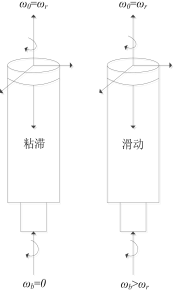
\includegraphics[width=0.35\linewidth]{figures/钻柱粘滑振动示意图}
		\caption{钻柱粘滑振动示意图}
		\label{fig:钻柱粘滑振动示意图}
	\end{figure}
	
	
	\autoref{fig:钻柱粘滑振动示意图} 中,$\omega _0$ 为钻柱的角速度,${\omega _r}$ 为旋转转盘的角速度,${\omega _b}$为钻头的角速度。图中钻柱的角速度${\omega_0}$始终与转盘的角速度${\omega _r}$ 相等,当井下岩石与钻头之间的摩擦力矩大于旋转转盘传递到钻头的驱动扭矩时,钻头的角速度为零,即${\omega _b}=0$ ,钻头由于无法转动而处于粘滞状态,此时转盘的角速度不变,还为${\omega _r}$;而转盘与钻柱此时还在继续转动,由钻 柱传递到钻头上的驱动扭矩也一直积聚在钻头上,当积聚在钻头上的驱动扭矩远远大于 钻头与岩石间的摩擦力矩时,钻头角速度由零开始快速增加到最大值,钻头摆脱粘滞状 态,此时钻头与岩石的运动状态为滑动状态,且${\omega _b} > {\omega _r}$;当钻头高速旋转回到正常状态 后,积聚在钻头上的驱动扭矩慢慢释放,又会小于钻头与岩石之间产生的摩擦力矩,此 时钻头的角速度${\omega _r}=0$,钻头又处于粘滞状态。如此反复出现粘滞与滑动过程,即为钻柱 的粘滑振动现象。
	
	
	
	\iffalse
	\subsection{插入表格}
	本模板文件如表~\ref{doc} 所示。
	\begin{table}[!htbp]
		\centering
		\caption{本模板文件组成}
		\renewcommand{\arraystretch}{1.25} % 增加行间距  
		\begin{tabular}{c@{\hspace{20pt}}c} % 增加列间距  
			
			\hline
			文件名 & 说明 \\
			\hline
			\texttt{main.tex}  & 主文件 \\
			\texttt{reference.bib} & 参考文献 \\
			\texttt{BUAAReport.sty}  & 文档格式控制\\
			\texttt{figures}  & 图片文件夹 \\
			\texttt{code}  & 代码文件夹 \\
			\hline
		\end{tabular}
		\label{doc}
	\end{table}
	
	\fi
	

	\begin{algorithm*}[H]
		\caption{钻进参数推荐控制逻辑(简化版)}
		\KwIn{cluster: 当前地层硬度聚类(1:软, 2:中, 3:硬)\\
			\hspace{2.5em}kr: 当前给进阻尼}
		\KwOut{set\_speed: 推荐给进速度\\
			\hspace{2.5em}set\_rpm: 推荐转速}
		
		\If{cluster == 1}{
			set\_speed $\gets$ 13, set\_rpm $\gets$ 160\;
			\If{kr $<$ 1.0}{
				set\_speed $\gets$ set\_speed + 2,set\_rpm $\gets$ set\_rpm + 10\;
				
			}
			\ElseIf{kr $<$ 3.0}{
				set\_speed $\gets$ set\_speed + 1,
				set\_rpm $\gets$ set\_rpm + 5,
			}
			\Else{
				set\_speed $\gets$ set\_speed - 1,
				set\_rpm $\gets$ set\_rpm - 5,
			}
		}
		\ElseIf{cluster == 2}{
			set\_speed $\gets$ 10,
			set\_rpm $\gets$ 150\;
			\If{kr $<$ 1.0}{
				set\_speed $\gets$ set\_speed + 2,
				set\_rpm $\gets$ set\_rpm + 10,
			}
			\ElseIf{kr $<$ 3.0}{
				set\_speed $\gets$ set\_speed + 1,
				set\_rpm $\gets$ set\_rpm + 5,
			}
			\Else{
				set\_speed $\gets$ set\_speed - 1,
				set\_rpm $\gets$ set\_rpm - 5,
			}
		}
		\ElseIf{cluster == 3}{
			set\_speed $\gets$ 8,
			set\_rpm $\gets$ 140\;
			\If{kr $<$ 1.0}{
				set\_speed $\gets$ set\_speed + 2,
				set\_rpm $\gets$ set\_rpm + 10\;
			}
			\ElseIf{kr $<$ 3.0}{
				set\_speed $\gets$ set\_speed + 1,
				set\_rpm $\gets$ set\_rpm + 5\;
			}
			\Else{
				set\_speed $\gets$ set\_speed - 1,
				set\_rpm $\gets$ set\_rpm - 5,
			}
		}
	\end{algorithm*}
	
	\section{钻柱系统的建模}
	在上一章中对钻柱系统的组成及各种原理进行了描述,本章主要讲述钻柱系统动力 学模型的建立。由于钻柱系统的复杂程度过高,其动力学模型的建立难度过大,但为了 能对钻柱系统进行系统分析,必须先对钻柱系统进行结构简化,合理的简化不会影响对 钻柱系统的分析,所以对简化后的钻柱系统进行动力学建模是可取的。对钻柱系统的结构简化通常会分为低自由度和多自由度模型,研究领域大多将其简化为两自由度和四自 由度,两自由度一般分为旋转转盘和钻头两部分,四自由度一般包含旋转转盘、钻杆、井底钻具组合(BHA)和井底钻头四部分。本章将钻柱系统简化为四自由度模型,分别 对旋转转盘、钻杆、BHA 和井底钻头建立动力学方程。
	\subsection{钻柱系统的结构简化}
	钻柱系统主要由井架、天车、游车、大钩、方钻杆、绞车、转盘、钻杆、钻铤和钻 头组成,为了便于钻柱粘滑振动的研究,将钻柱系统简化为四个部分:(1)转盘;(2) 钻杆;(3)BHA;(4)钻头。在此需要给出以下几个假设条件:
	
	(1)该钻柱系统必须处于垂直井中;
	
	(2)不考虑钻柱的横向振动轴向振动;
	
	(3)不考虑钻杆与井壁之间的摩擦阻力对钻井过程的影响;
	
	(4)不考虑钻井液对钻柱产生的影响;
	
	(5)对井下岩石的强度变化忽略不计。
	
	根据以上五条假设条件,钻柱系统的动力学简化模型如\autoref{fig:钻柱系统简化模型} 所示。
	
	
	\begin{figure}[!htbp]
		\centering
		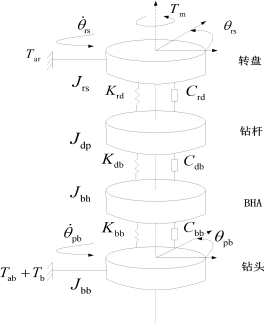
\includegraphics[width=0.5\linewidth]{figures/钻柱系统简化模型}
		\caption{钻柱系统简化模型}
		\label{fig:钻柱系统简化模型}
	\end{figure}
	
	
	钻柱简化模型图中转盘、钻杆、BHA 以及钻头之间均通过具有扭转刚度和扭转阻尼 的线性弹簧连接。在钻井过程中,转盘驱动系统带动旋转转盘转动,转盘通过带动方钻 杆使 BHA 转动,BHA 进而带动井下钻头转动来破碎岩石和钻进。
	由\autoref{fig:钻柱系统简化模型} 钻柱系统的简化模型可得钻柱系统的运动微分方程如下:
	\begin{equation}
		\left\{ \begin{array}{l}
			{J_{rs}}{{\ddot \theta }_{rs}} + {K_{rd}}({\theta _{rs}} - {\theta _{dp}}) + {C_{rd}}({{\dot \theta }_{rs}} - {{\dot \theta }_{dp}}) - {T_m} + {T_{ar}} = 0\\
			{J_{dp}}{{\ddot \theta }_{dp}} - {K_{rd}}({\theta _{rs}} - {\theta _{dp}}) + {K_{db}}({\theta _{dp}} - {\theta _{dh}}) - {C_{rd}}({{\dot \theta }_{rs}} - {{\dot \theta }_{dp}}) + {C_{db}}({{\dot \theta }_{dp}} - {{\dot \theta }_{bh}}) = 0\\
			{J_{bh}}{{\ddot \theta }_{bh}} - {K_{db}}({\theta _{dp}} - {\theta _{bh}}) + {K_{bb}}({\theta _{bh}} - {\theta _{pb}}) - {C_{db}}({{\dot \theta }_{dp}} - {{\dot \theta }_{bh}}) + {C_{bb}}({{\dot \theta }_{bh}} - {{\dot \theta }_{pb}}) = 0\\
			{J_{bb}}{{\ddot \theta }_{bb}} - {K_{bb}}({\theta _{bh}} - {\theta _{pb}}) - {C_{bb}}({{\dot \theta }_{bh}} - {{\dot \theta }_{pb}}) - {T_{ab}} + {T_b} = 0
		\end{array} \right.
		\label{eq:钻柱系统的运动微分方程}
	\end{equation}
	
	\autoref{eq:钻柱系统的运动微分方程} 中 $J_{rs}, J_{dp}, J_{bh},J_{bb}$分别为转盘,钻杆,BHA和钻头的转动惯量,${\rm{kg}} \cdot {{\rm{m}}^{\rm{2}}}$;${\ddot \theta }_{rs}, {\ddot \theta }_{dp}, {\ddot \theta }_{bh}, {\ddot \theta }_{bb}, $ 分别为转盘,钻杆,BHA 和钻头的角加速度,${\rm{rad/}}{{\rm{s}}^2}$;$K_{rd}, K_{db}, K_{bb}$分别为转盘 与钻杆,钻杆与 BHA ,BHA 与钻头之间的弹簧扭转刚度,N·m/rad;$\theta_{rs}, \theta_{dp}, \theta_{bh}, \theta_{pb}$分别为转盘,钻杆,BHA 和钻头的角位移,rad;$C_{rd} , C_{db}, C_{bb}$分别为转盘与钻杆,钻杆与 BHA ,BHA 与钻头之间的弹簧扭转阻尼,N·m · s/rad;$\dot \theta_{rs}, \dot \theta_{dp}, \dot \theta_{bh}, \dot \theta_{pb}$ 分别为转盘,钻杆,BHA 和钻头的角速度,rad/s;$T_m$ 为转盘的驱动扭矩;$T_{ar}$ 为旋转系统的粘性阻尼力矩,表达式为:
	\begin{equation}
		{T_{ar}} = {C_{rs}}{{\dot \theta }_{rs}}
	\end{equation}
	式中 $C_{rs}$ 为转盘粘性阻尼系数。$T_{ab}$为钻头上的粘性阻尼力矩,表达式为:
	\begin{equation}
		{T_{ab}} = {C_{pb}}{{\dot \theta }_{pb}}
	\end{equation}
	式中 $C_{pb}$ 为钻头的粘滞阻尼。$T_b$ 为钻头上的摩擦力矩,由于钻头在切削岩石时所 受摩擦力矩的不同,摩擦力矩 $T_b$ 可用三段式方程表示,钻头摩擦力矩如图 3-2 ,表达式 为:                                  
	\begin{equation}
		{T_b} = \left\{ {\begin{array}{*{20}{l}}
				{{T_r}}&{if\left| {{{\dot \theta }_{pb}}} \right| < \xi \& \left| {{T_r}} \right| \le {T_s}}\\
				{{T_s}sign({T_r})}&{if\left| {{{\dot \theta }_{pb}}} \right| < \xi \& \left| {{T_r}} \right| > {T_s}}\\
				{{T_b} = {W_b}{R_b}{\mu _b}sign({{\dot \theta }_{pb}})}&{if\left| {{{\dot \theta }_{pb}}} \right| > {\xi _s}}
		\end{array}} \right.
	\end{equation}
	
	式中 $Tr$ 为施加在钻头上的扭矩,N·m ,$\xi$为一个接近于零的正数;当钻头的角速度${\left| {{{\dot \theta }_{pb}}} \right|} < \xi $  且积聚在钻头上的驱动扭矩${\left| {{T_r}} \right| }\le {T_s}$时,说明钻头此时所受的摩擦力矩大于由钻柱传递来的驱动扭矩,钻头处于粘滞状态,此时:
	
	\begin{equation}
		{T_b} = {T_r} = {K_{bb}}({\theta _{bh}} - {\theta _{pb}}) + {C_{bb}}({{\dot \theta }_{bh}} - {{\dot \theta }_{pb}}) - {T_{ab}}
	\end{equation}
	$T_s$ 为钻头与岩石之间相互作用产生的最大静摩擦扭矩,N·m ,表达式为: 
	
	
	\begin{equation}
		T_s  = W_bR_b\mu _{sb}
	\end{equation}
	
	
	
	式中 $W_b$ 为钻压,N;$R_b$ 为钻头的半径,m;$\mu _{sb}$为静摩擦系数。当钻头角速度${\left| {{{\dot \theta }_{pb}}} \right| > {\xi _s}}$ 时,说明钻头此时积聚的驱动扭矩大于与岩石之间的摩擦力矩,钻头处于滑动状态,此时:
	\begin{equation}
		T_b  = W_bR_b\mu _bsign (\dot\theta  _{pb})  
	\end{equation}
	
	
	
	\begin{figure}
		\centering
		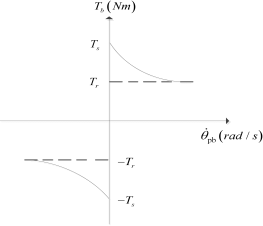
\includegraphics[width=0.7\linewidth]{figures/钻头摩擦力矩}
		\caption[钻头摩擦力矩]{}
		\label{fig:钻头摩擦力矩}
	\end{figure}
	
	
	$\mu _b$ 为干摩擦系数,表达式为:
	\begin{equation}
		\mu_b = \mu_{cb} + (\mu_{sb} - \mu_{cb})e^{-\gamma_b\theta_{bb}}
	\end{equation}                                                                         $\mu_{cb}$为钻头的库伦摩擦系数,并且$\gamma_b$ 为小于 1 的正数;$\mu_{sb}$为静摩擦系数。
	将式(3-2)和(3-3)代入式(3-1)中,可将钻柱系统的运动微分方程改写为下式:
	
	\begin{equation}
		\left\{ \begin{array}{l}
			{J_{rs}}{{\ddot \theta }_{rs}} + {K_{rd}}({\theta _{rs}} - {\theta _{dp}}) + {C_{rd}}({{\dot \theta }_{rs}} - {{\dot \theta }_{dp}}) - {T_m} + {C_{rs}}{{\dot \theta }_{rs}} = 0\\
			{J_{dp}}{{\ddot \theta }_{dp}} - {K_{rd}}({\theta _{rs}} - {\theta _{dp}}) + {K_{db}}({\theta _{dp}} - {\theta _{dh}}) - {C_{rd}}({{\dot \theta }_{rs}} - {{\dot \theta }_{dp}}) + {C_{db}}({{\dot \theta }_{dp}} - {{\dot \theta }_{bh}}) = 0\\
			{J_{bh}}{{\ddot \theta }_{bh}} - {K_{db}}({\theta _{dp}} - {\theta _{bh}}) + {K_{bb}}({\theta _{bh}} - {\theta _{pb}}) - {C_{db}}({{\dot \theta }_{dp}} - {{\dot \theta }_{bh}}) + {C_{bb}}({{\dot \theta }_{bh}} - {{\dot \theta }_{pb}}) = 0\\
			{J_{bb}}{{\ddot \theta }_{bb}} - {K_{bb}}({\theta _{bh}} - {\theta _{pb}}) - {C_{bb}}({{\dot \theta }_{bh}} - {{\dot \theta }_{pb}}) - {C_{pb}}{{\dot \theta }_{pb}} + {T_b} = 0
		\end{array} \right.
		\label{钻柱系统的运动微分方程改写}
	\end{equation}
	
	\subsection{钻柱系统动力学建模}
	根据钻柱系统简化模型及公式(3-8)可得模型中各部分的角加速度公式如下: 
	\begin{equation}
		\left\{ \begin{array}{l}
			{\ddot \theta_{rs}} = -\dfrac{K_{rd}}{J_{rs}}(\theta_{rs} - \theta_{dp}) - \dfrac{C_{rd}}{J_{rs}}(\dot \theta_{rs} - \dot \theta_{dp}) + \dfrac{T_m}{J_{rs}} - \dfrac{C_{rs}}{{\dot \theta }_{rs}}{J_{rs}} \\
			{\ddot \theta_{dp}} = \dfrac{K_{rd}}{J_{dp}}(\theta_{rs} - \theta_{dp}) - \dfrac{K_{db}}{J_{dp}}(\theta_{dp} - \theta_{dh}) + \dfrac{C_{rd}}{J_{dp}}(\dot \theta_{rs} - \dot \theta_{dp}) - \dfrac{C_{db}}{J_{dp}}(\dot \theta_{dp} - \dot \theta_{bh}) \\
			{\ddot \theta_{bh}} = \dfrac{K_{db}}{J_{bh}}(\theta_{dp} - \theta_{bh}) - \dfrac{K_{bb}}{J_{bh}}(\theta_{bh} - \theta_{pb}) + \dfrac{C_{db}}{J_{bh}}(\dot \theta_{dp} - \dot \theta_{bh}) - \dfrac{C_{bb}}{J_{bh}}(\dot \theta_{bh} - \dot \theta_{pb}) \\
			{\ddot \theta_{bb}} = \dfrac{K_{bb}}{J_{bb}}(\theta_{bh} - \theta_{pb}) + \dfrac{C_{bb}}{J_{bb}}(\dot \theta_{bh} - \dot \theta_{pb}) + \dfrac{C_{pb}}{J_{bb}} \dot \theta_{pb} - \dfrac{T_b}{J_{bb}} 
		\end{array} \right.
	\end{equation}
	
	为了便于计算,令 $T_m =u$ ,并令 $x_1  = \dot \theta_{rs}, x_2  = \theta_{rs} -  \theta_{dp},x_3  = \theta_{dp}, x_4  = \theta_{dp} -  \theta_{bh}, x_5  = \dot \theta_{dh}, x_6  = \theta_{bh} -  \theta_{pb}, x_2  = \dot \theta_{pb}$为系统状态变量,代入式中,可得钻柱系统的状态空间方程:
	
	\begin{equation}
		\left\{ {\begin{array}{*{20}{l}}
				{\mathop {{x_1}}\limits^.  = \dfrac{{ - ({C_{rd}} + {C_{rd}})}}{{{J_{rs}}}}{x_1} - \dfrac{{{K_{rd}}}}{{{J_{rs}}}}{x_2} + \dfrac{{{C_{rs}}}}{{{J_{rs}}}}{x_3} + \dfrac{u}{{{J_{rs}}}}}\\
				{\mathop {{x_2}}\limits^.  = {x_1} - {x_3}}\\
				{\mathop {{x_3}}\limits^.  = \dfrac{{{C_{rd}}}}{{{J_{dp}}}}{x_1} + \dfrac{{{K_{rd}}}}{{{J_{dp}}}}{x_2} - \dfrac{{({C_{bb}} + {C_{db}})}}{{{J_{dp}}}}{x_3} - \dfrac{{{K_{db}}}}{{{J_{dp}}}}{x_4} + \dfrac{{{C_{db}}}}{{{J_{dp}}}}{x_5}}\\
				{\mathop {{x_4}}\limits^.  = {x_3} - {x_5}}\\
				{\mathop {{x_5}}\limits^.  = \dfrac{{{C_{db}}}}{{{J_{bh}}}}{x_3} + \dfrac{{{K_{db}}}}{{{J_{bh}}}}{x_4} - \dfrac{{({C_{bb}} + {C_{db}})}}{{{J_{bh}}}}{x_5} - \dfrac{{{K_{bb}}}}{{{J_{bh}}}}{x_6} + \dfrac{{{C_{bb}}}}{{{J_{bh}}}}{x_7}}\\
				{\mathop {{x_6}}\limits^.  = {x_5} - {x_7}}\\
				{\mathop {{x_7}}\limits^.  = \dfrac{{{C_{bb}}}}{{{J_{bb}}}}{x_5} + \dfrac{{{K_{bb}}}}{{{J_{bb}}}}{x_6} - \dfrac{{({C_{bb}} + {C_{db}})}}{{{J_{bb}}}}{x_7} - \dfrac{{{T_b}}}{{{J_{bb}}}}}
		\end{array}} \right.
	\end{equation}
	
	可简化为:
	\begin{equation}
		\begin{cases} \dot{x}(t)=Ax(t)+Bu(t)+B_{1}d(t)\\ y(t)=Cx(t) \end{cases} 
	\end{equation}
	
	
	式中$A, B$ 为状态方程系数矩阵,由系统参数决定;因为只有钻柱系统顶部的参数可以测量,所以$ y(t)$是转盘转速,
	输入量$u(t) = T_r$,扰动量为$d(t)=T_b$                 
	
	\begin{align*} & A=\begin{bmatrix} -J^{-1}(C_{1}+C_{2}) & J^{-1}a_{1}\\ a_{2} & O_{n-1\times n-1} \end{bmatrix}\\ & a_{1}=\begin{bmatrix} -k_{p} & 0 & \cdots & 0 \\ k_{p} & -k_{p} & \cdots & 0\\ \vdots & \ddots & \ddots & \vdots\\ 0 & \cdots & k_{r} & -k_{b}\\ 0 & \cdots & 0 & k_{b} \end{bmatrix}\\ & a_{2}=\begin{bmatrix} 1 & -1 & 0 & \cdots & 0\\ 0 & \ddots & \ddots & \ddots & 0\\ \vdots & \ddots & \ddots & \ddots & 0\\ 0 & \cdots & 0 & 1 & -1 \end{bmatrix}\\ & B=\begin{bmatrix} J^{-1}S_{r}\\ O_{n-1\times 1} \end{bmatrix}\ B_{1}=\begin{bmatrix} J^{-1}S_{b}\\ O_{n-1\times 1} \end{bmatrix}\ C=\begin{bmatrix} 1\\ O_{2n-2\times 1} \end{bmatrix}^{T} \end{align*}
	本次实验取n=7,状态空间模型的阶数是 2n。对于实际的钻弦系统,n 趋于无穷大。因此,多自由度模型可以保证钻柱系统的建模精度\cite{chengjun}。
	
	
	
	
	\subsection{钻柱系统仿真模型的建立}
	粘滑振动的抑制问题可以看作是钻头速度的跟踪控制问题。同时,由于只能进行表面测量,因此基于观察者的控制方法适用于这种情况。因此,本节介绍了一种基于零稳态误差和状态观测器的跟踪控制和控制系统。
	
	控制系统的结构如图 1 所示,分别包括钻柱动力学模型、内部模型、状态反馈和状态观测器。钻探动态模型已在 (5) 中描述。
	
	
	
	\begin{figure}[!htbp]
		\centering
		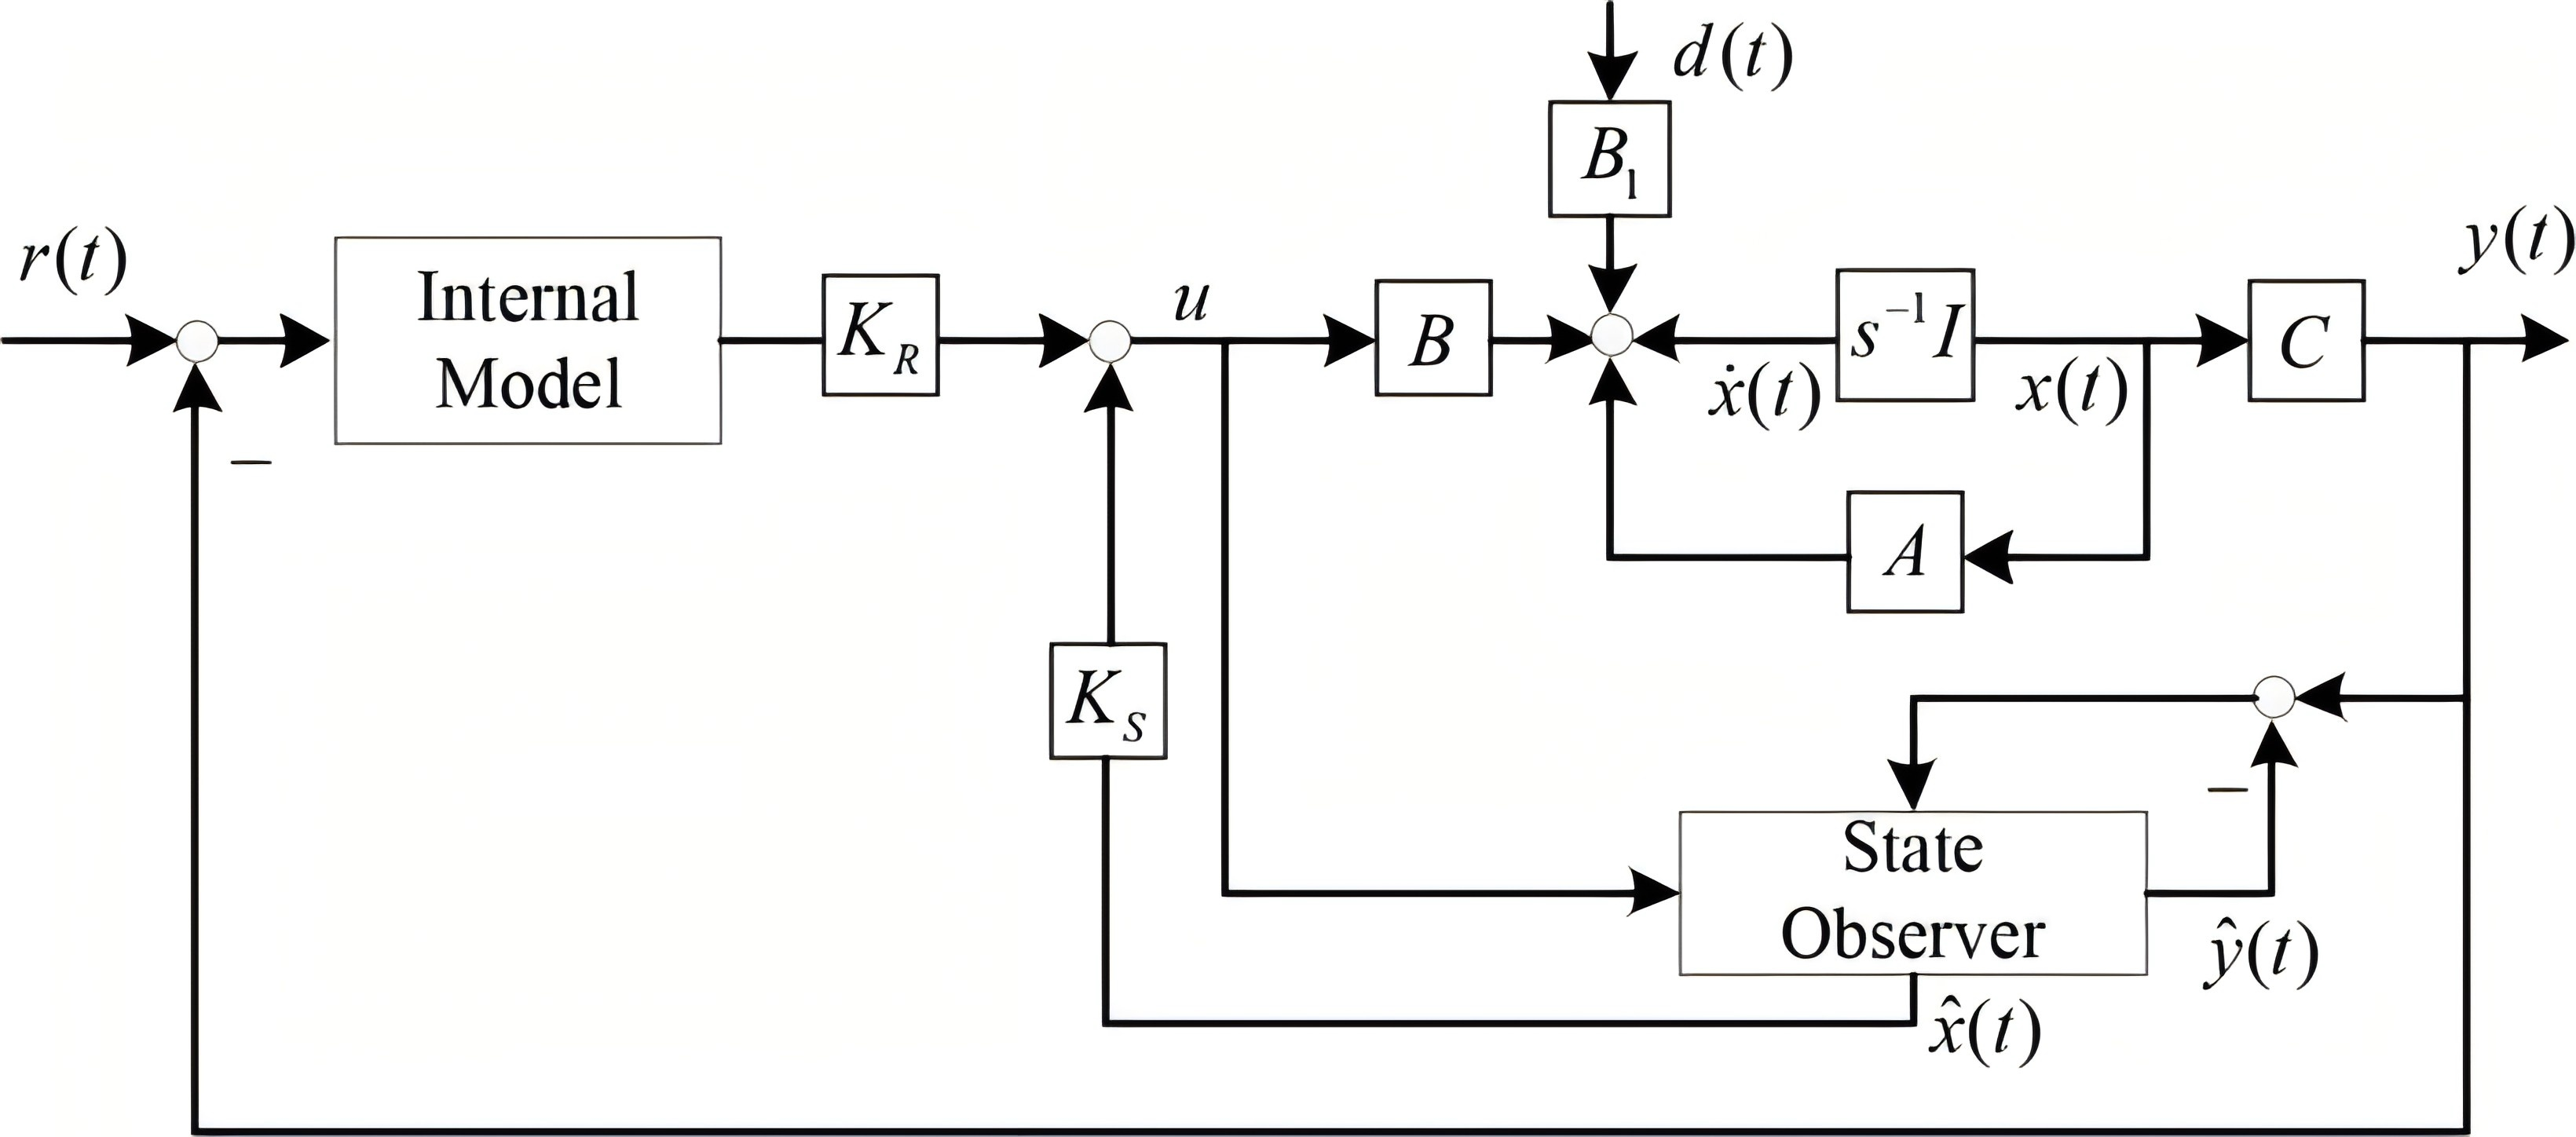
\includegraphics[width=0.7\linewidth]{figures/控制系统结构}
		\caption{控制系统结构}
		\label{fig:控制系统结构}
	\end{figure}
	
	参考输入和干扰的内部模型如下所示:
	\begin{equation} 
		\begin{cases} \dot{x}_{c}(t)=A_{c}x_{c}(t)+B_{c}e(t)\\ y_{c}(t)=C_{c}x_{c}(t) \end{cases}  
	\end{equation}
	
	表示内模和钻柱模型的增广矩阵为:
	\begin{align} {\bar{x}}(t)& = {[x(t){\rm{\;}}{x_c}(t)]^T} \\ \dot{\bar{x}}(t) & =\bar{A}\bar{x}(t)+\bar{B}u(t)+\bar{B}_{1}d(t)\\ & =\begin{bmatrix} A & 0\\ -B_{c}C & A_{c} \end{bmatrix}\bar{x}(t)+\begin{bmatrix} B\\ 0 \end{bmatrix}u(t)+\begin{bmatrix} B_{1}\\ 0 \end{bmatrix}d(t)  \end{align}
	
	输入:
	\begin{equation}
		u(t)=-\bar{K}\bar{x}(t)=[-K_{S}\quad K_{R}]\bar{x}(t)
	\end{equation}
	
	$K_S$和$K_R$分别是状态反馈增益和内模增益。
	
	
	
	然而,在实际钻孔过程中,只有顶部测量可用,这使得基于全状态反馈的控制变得不可能。因此,全维状态观测器用于估计钻柱系统中的状态,并被描述为:
	\begin{equation}
		\dot{\hat{x}}(t)=A\hat{x}(t)+Bu(t)+L(y(t)-\hat{y}(t))\\ \hat{y}(t)=C\hat{x}(t)
	\end{equation}
	${\hat{x}}(t)$是${x}(t)$的状态观测值,$L$是增益矩阵。
	
	结合状态观测器,输入为:
	\begin{equation}
		u(t)=[-K_{S}\quad K_{R}]\begin{bmatrix} \hat{x}(t)\\ \hat{x}_{c}(t) \end{bmatrix} 
	\end{equation}
	
	\begin{table}[htbp!]
		\centering
		\caption{钻柱系统相关参数}
		\begin{tabular}{cc} 
			\toprule
			参数                                                 & 数值      \\ 
			\hline
			转盘转动惯量~${J}_{rs}$ $(kg·m^2)$               & 930     \\
			钻杆转动惯量~${J}_{dp}$ $(kg·m^2)$               & 2782    \\
			BHA~转动惯量~${J}_{bh} $ $(kg·m^2)$             & 750     \\
			钻头转动惯量~${J}_{bb}$ $(kg·m^2)$               & 472     \\
			转盘与钻杆之间弹簧扭转刚度~${K}_{rd}$ $(N·m/rad)$      & 698     \\
			钻杆与~BHA~之间弹簧扭转刚度~${K}_{db}$ $(N·m/rad)$   & 1080    \\
			BHA~与钻头之间弹簧扭转刚度~${K}_{bb}$ $(N·m/rad)$    & 907     \\
			转盘与钻杆之间弹簧扭转阻尼~${C}_{rd}$ $(N·m~·s/rad)$   & 140     \\
			钻杆与~BHA~之间弹簧扭转阻尼~${C}_{db}$ $(N·m~·s/rad)$& 190     \\
			BHA~与钻头之间弹簧扭转阻尼~${C}_{bb}$ $(N·m~·s/rad)$ & 181     \\
			转盘粘性阻尼系数~${C}_{rs}$ $(N·m~·s/rad)$        & 425     \\
			钻头粘滞阻尼系数~${C}_{pb}$ $(N·m~·s/rad)$        & 50      \\
			钻压~${W}_b~$ ${(N)}$                        & 97347   \\
			给定转速~$V$ $(rad/s) $                            & 12      \\
			钻头半径~${R}b$ ${(m)} $                      & 0.1555  \\
			库伦摩擦因数${\mu _{cb}} $                                & 0.5     \\
			${\xi}$                                         & 10-6    \\
			${\mu _{sb}}$                                       & 0.8     \\
			${\gamma_b}  $                                      & 0.9     \\
			\bottomrule
		\end{tabular}
	\end{table}
	
	\newpage
	\section{钻柱系统仿真实验}
	本章主要对上一章所给出的运动微分方程进行仿真模型搭建,模拟钻柱系统在钻井过程中发生的粘滑振动现象,并设计相应的控制器抑制钻柱粘滑振动。
	
	
	\subsection{未加控制的钻柱模型}
	
	\subsubsection{Simulink仿真}
	未加控制的钻柱模型如下
	
	\begin{figure}[!htbp]
		\centering
		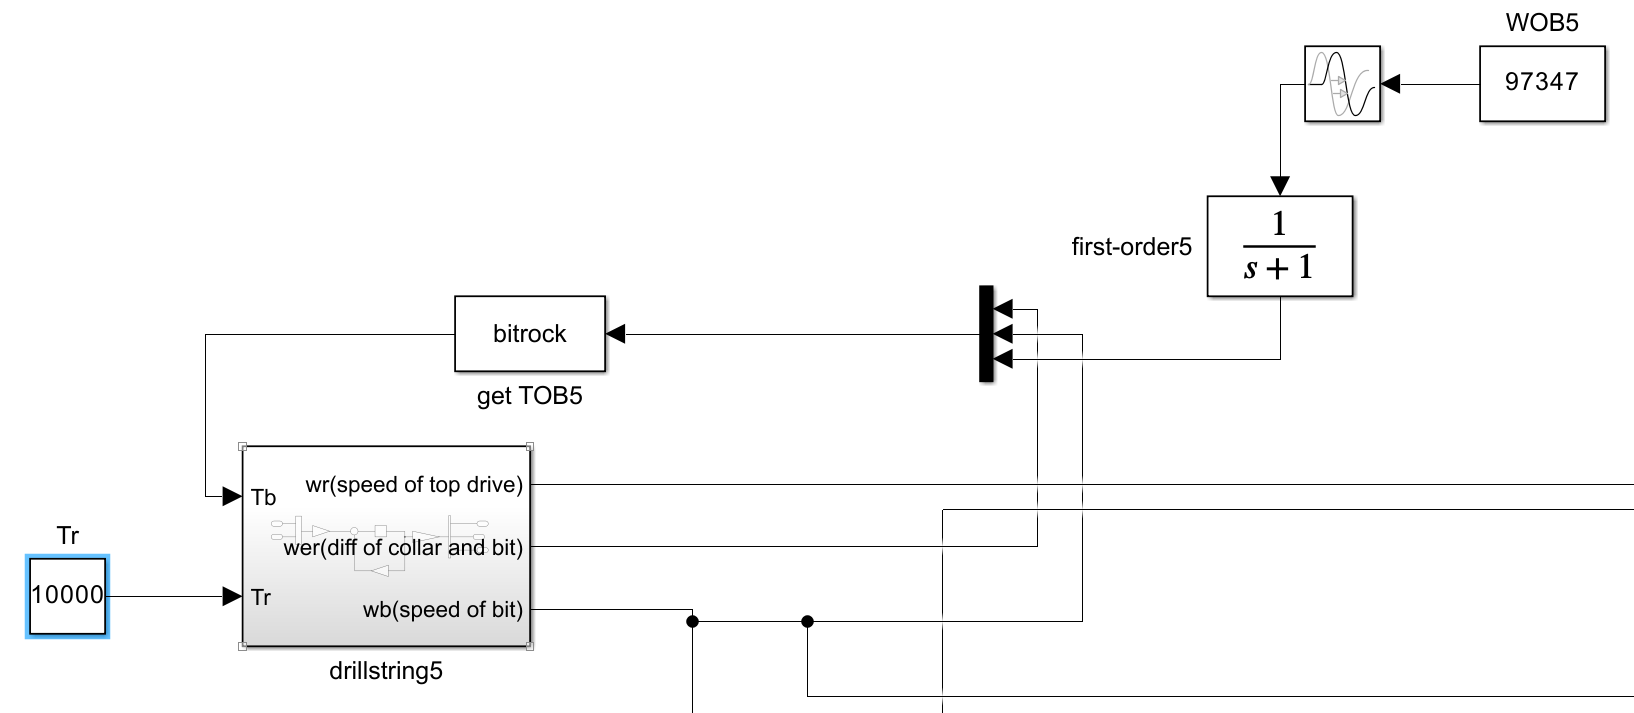
\includegraphics[width=0.6\linewidth]{figures/未加控制}
		\caption{未加控制的钻柱模型}
		\label{fig:未加控制}
	\end{figure}
	
	
	%钻柱子系统模型:
	
	\begin{figure}[!htbp]
		\centering
		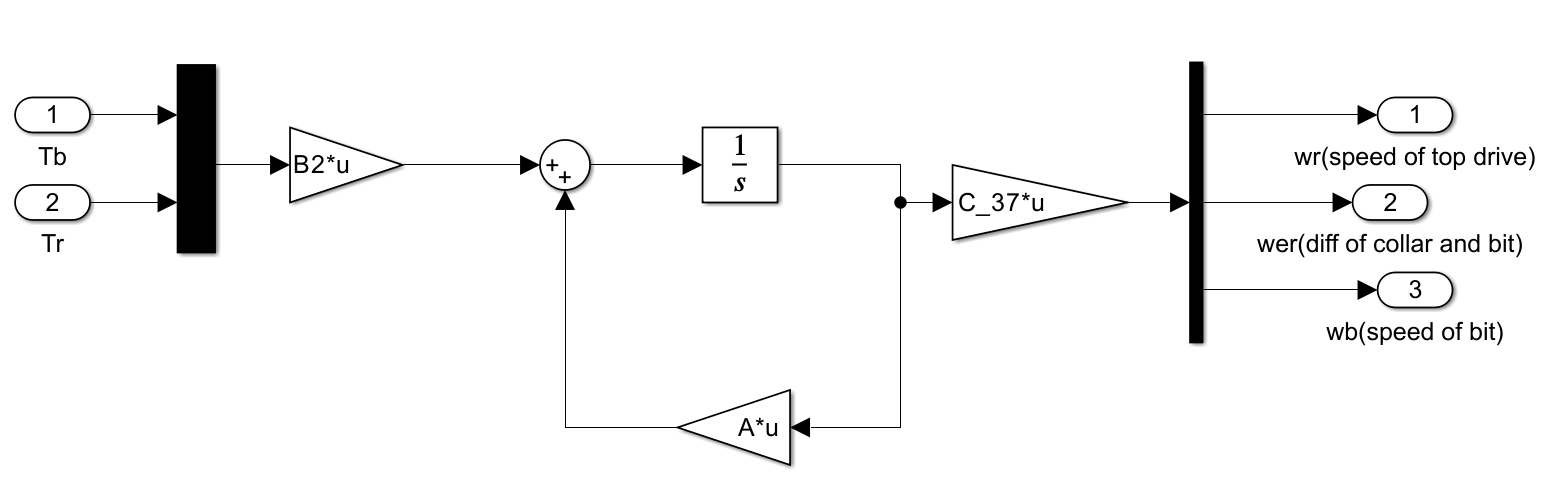
\includegraphics[width=0.6\linewidth]{figures/钻柱子系统}
		\caption{钻柱子系统模型}
		\label{fig:钻柱子系统}
	\end{figure}
	
	用Simulink模型仿真不加控制器时钻柱系统的Rotary Speed和Bit Speed粘滑振动如图 8 所示:
	
	\begin{figure}[!htbp]
		\centering
		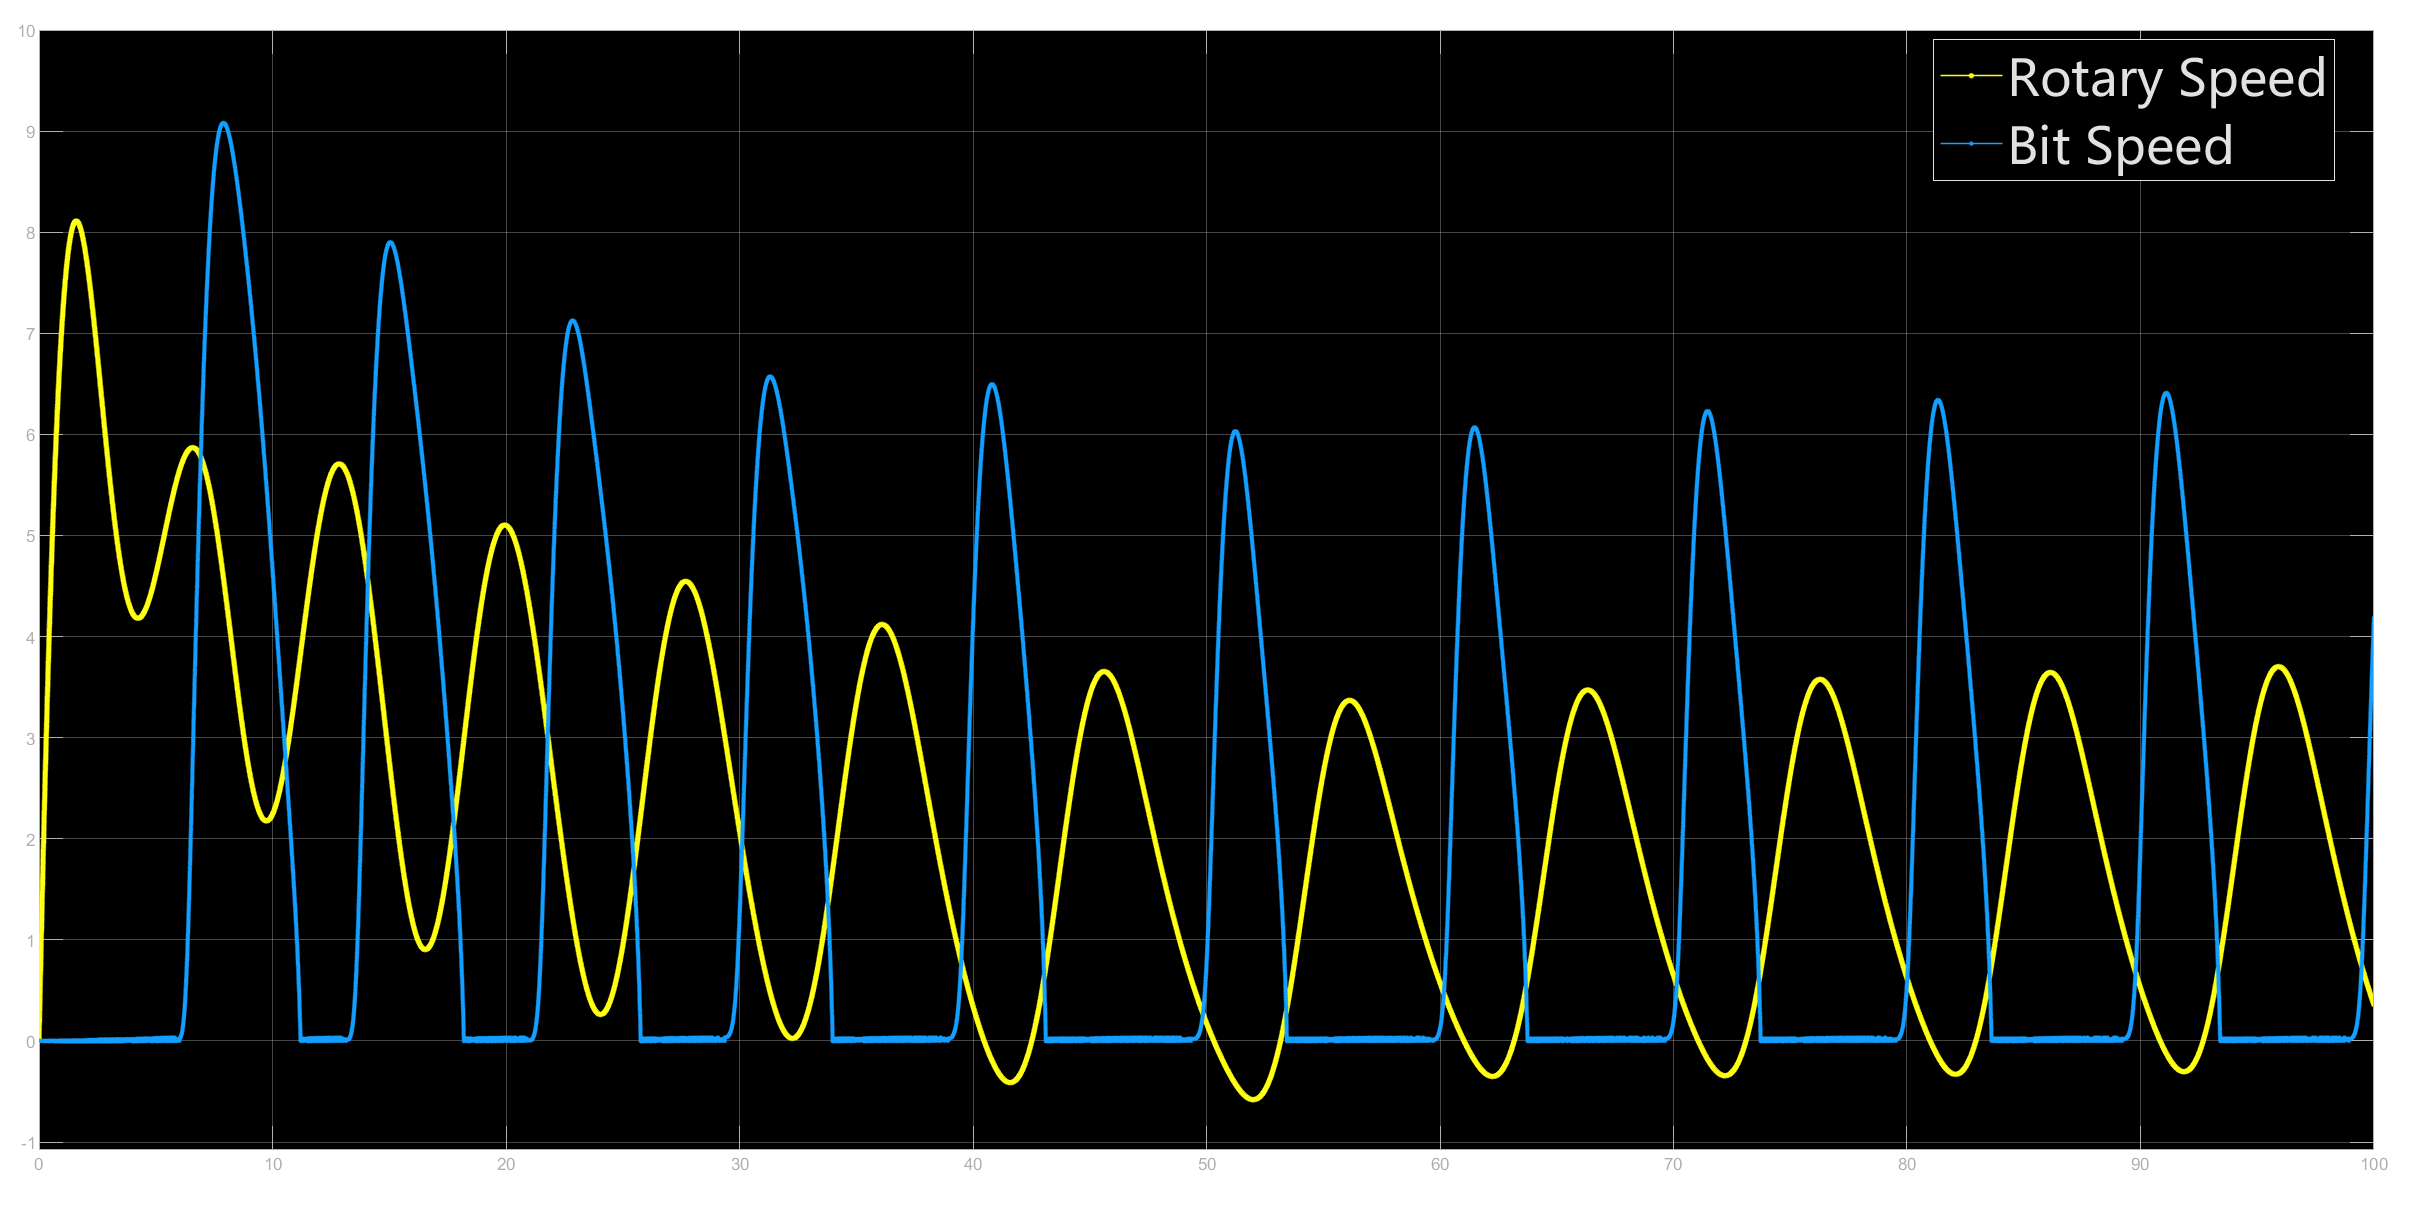
\includegraphics[width=0.7\linewidth]{figures/Rotary_Speed和Bit_Speed的粘滑振动}
		\caption{Rotary Speed和Bit Speed的粘滑振动}
		\label{fig:Rotary_Speed和Bit_Speed的粘滑振动}
	\end{figure}
	
	图 8 是钻压为 97.4kN 时的钻盘角速度和钻头角速度的变化曲线,保持其余钻井参数不变,分别将钻压 由 97.4kN 增大到 98.0kN 和 107.2kN。两种钻压下的钻头角速度变化曲线如图 \ref{fig:W_b=90kN和W_b=85kN 时钻头角速度的变化} 所示。由图可得,当钻压为 98.0kN 时,钻头仍然处于粘滞与滑动的周期性变化中,并没有因钻压的增大而发生其他变化;当钻压增大为 107.2kN 时,钻头出现持续的粘滞状态,没了滑动现象。
	
\begin{figure}[!htbp]
	\centering
	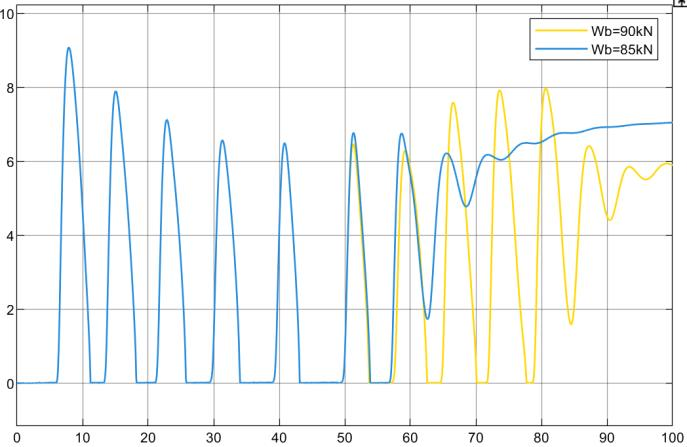
\includegraphics[width=0.6\linewidth]{figures/W_b=90kN和W_b=85kN 时钻头角速度的变化}
	\caption{$W_b$=90kN和$W_b$=85kN时钻头角速度的变化}
	\label{fig:W_b=90kN和W_b=85kN 时钻头角速度的变化}
\end{figure}
	
	
	
	
	保持其余钻井参数不变,将钻柱系统的钻压由 97.4kN 减小为 90kN,此时的钻头角速度变化曲线如图 \ref{fig:W_b=98kN和W_b=107.2kN 时钻头角速度的变化} 黄线所示。由图可得,当钻压减小时,钻头除了在Wb开始由钻柱带动旋转的时间内处于静止状态以外,钻头的角速度随着钻柱的带动迅速增大,然后由于钻头岩石的摩擦力矩影响又开始降低,随后又开始增加,经过几次增大减小后,最终稳定在6.0rad/s,并持续稳定。继续由97.4kN 减小到85kN,此时钻头的角速度变化曲线如图 4-3 蓝线所示。由图可得,当钻柱系统的钻压再次减小时,钻头的角速度在前期的变化和钻压值为 90kN 时一样,不一样的在于最终稳定状态时的钻头角速度为 7.0rad/s。
	
		\begin{figure}[!htbp]
		\centering
		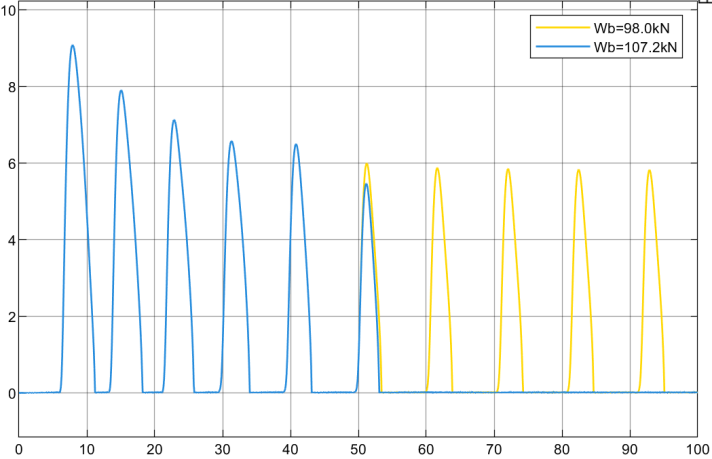
\includegraphics[width=0.6\linewidth]{figures/W_b=98kN和W_b=107.2kN 时钻头角速度的变化}
		\caption{$W_b$=98kN和$W_b$=107.2kN时钻头角速度的变化}
		\label{fig:W_b=98kN和W_b=107.2kN 时钻头角速度的变化}
	\end{figure}
	
	综合上述结果分析,增大钻柱系统的钻压并不能缓解钻柱粘滑振动,反而会增大粘滑振动的发生概率,过大的钻压会使钻头持续处于粘滞状态;相反适当的减小钻柱系统的钻压值,能够缓解钻柱粘滑振动的影响,也能够提高钻头的转速,但是仍然不能是钻头的角速度达到期望的速度。过小的钻压虽然能够缓解钻柱粘滑振动,但对于钻井作业的效率和钻机的切削深度会有较大的影响。在实际钻井作业时应用性不强。
	
	\subsubsection{用ode函数的求解比较}
	
	
	
	在 MATLAB 中,\texttt{ode45}、\texttt{ode23} 和 \texttt{ode15s} 是用于求解常微分方程(ODE)的不同函数,它们各自有不同的特点和适用场景。虽然在某些情况下,它们给出的结果可能相似,但它们的算法和适用性却有显著区别。%下面是对这三种方法的简要比较:  
	
	1. \texttt{ode45}  
	\begin{itemize}  
		\item 算法: 基于 Runge-Kutta 方法,特别是 Dormand-Prince 方法。  
		\item 适用情况: 通常用于一般的非刚性问题,适合大多数常见的 ODE。  
		\item 优点: 精度高,适合大多数问题,且使用简单。  
		\item 缺点: 对于刚性问题,可能会导致计算效率低下或不收敛。  
	\end{itemize}  
	
	2. \texttt{ode23}  
	\begin{itemize}  
		\item 算法: 基于低阶的 Runge-Kutta 方法,采用 2nd and 3rd order。  
		\item 适用情况: 适合较简单的非刚性问题,或者当你希望计算速度更快时。  
		\item 优点: 计算速度较快,适合对精度要求不高的情况。  
		\item 缺点: 精度低于 \texttt{ode45},在需要较高精度的情况下可能不够用。  
	\end{itemize}  
	
	3. \texttt{ode15s}  
	\begin{itemize}  
		\item 算法: 基于隐式方法,适合求解刚性(stiff)微分方程。  
		\item 适用情况: 特别适用于刚性问题,或者当系统的动态变化速度非常快时。  
		\item 优点: 在处理刚性问题时,计算效率更高,能够稳定收敛。  
		\item 缺点: 对于非刚性问题,可能会比 \texttt{ode45} 和 \texttt{ode23} 更慢。  
	\end{itemize}
	
	\newpage
	用ode45函数求解的Rotary Speed和Bit Speed的粘滑振动现象如\autoref{fig:ode45}所示。
	
	\begin{figure}[!htbp]
		\centering
		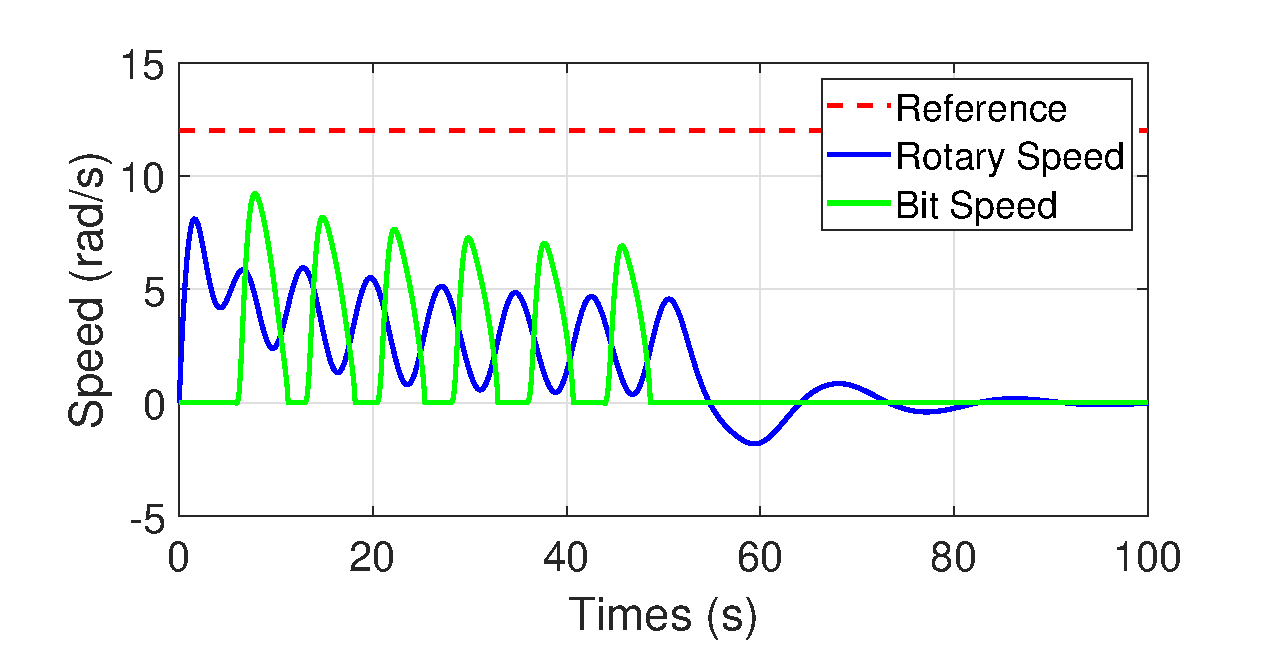
\includegraphics[width=0.7\linewidth]{figures/ode45}
		\caption{ode45}
		\label{fig:ode45}
	\end{figure}
	
	可见和simulink模型的仿真效果差不多。
	
	下面比较 ode45、ode23、ode15s 等MATLAB 函数。在给定转盘控制力矩时,求解钻柱粘滑振动微分方程,仿真钻柱粘滑振动现象,求解所得的Rotary speed如图:
	
	\begin{figure}[!htbp]
		\centering
		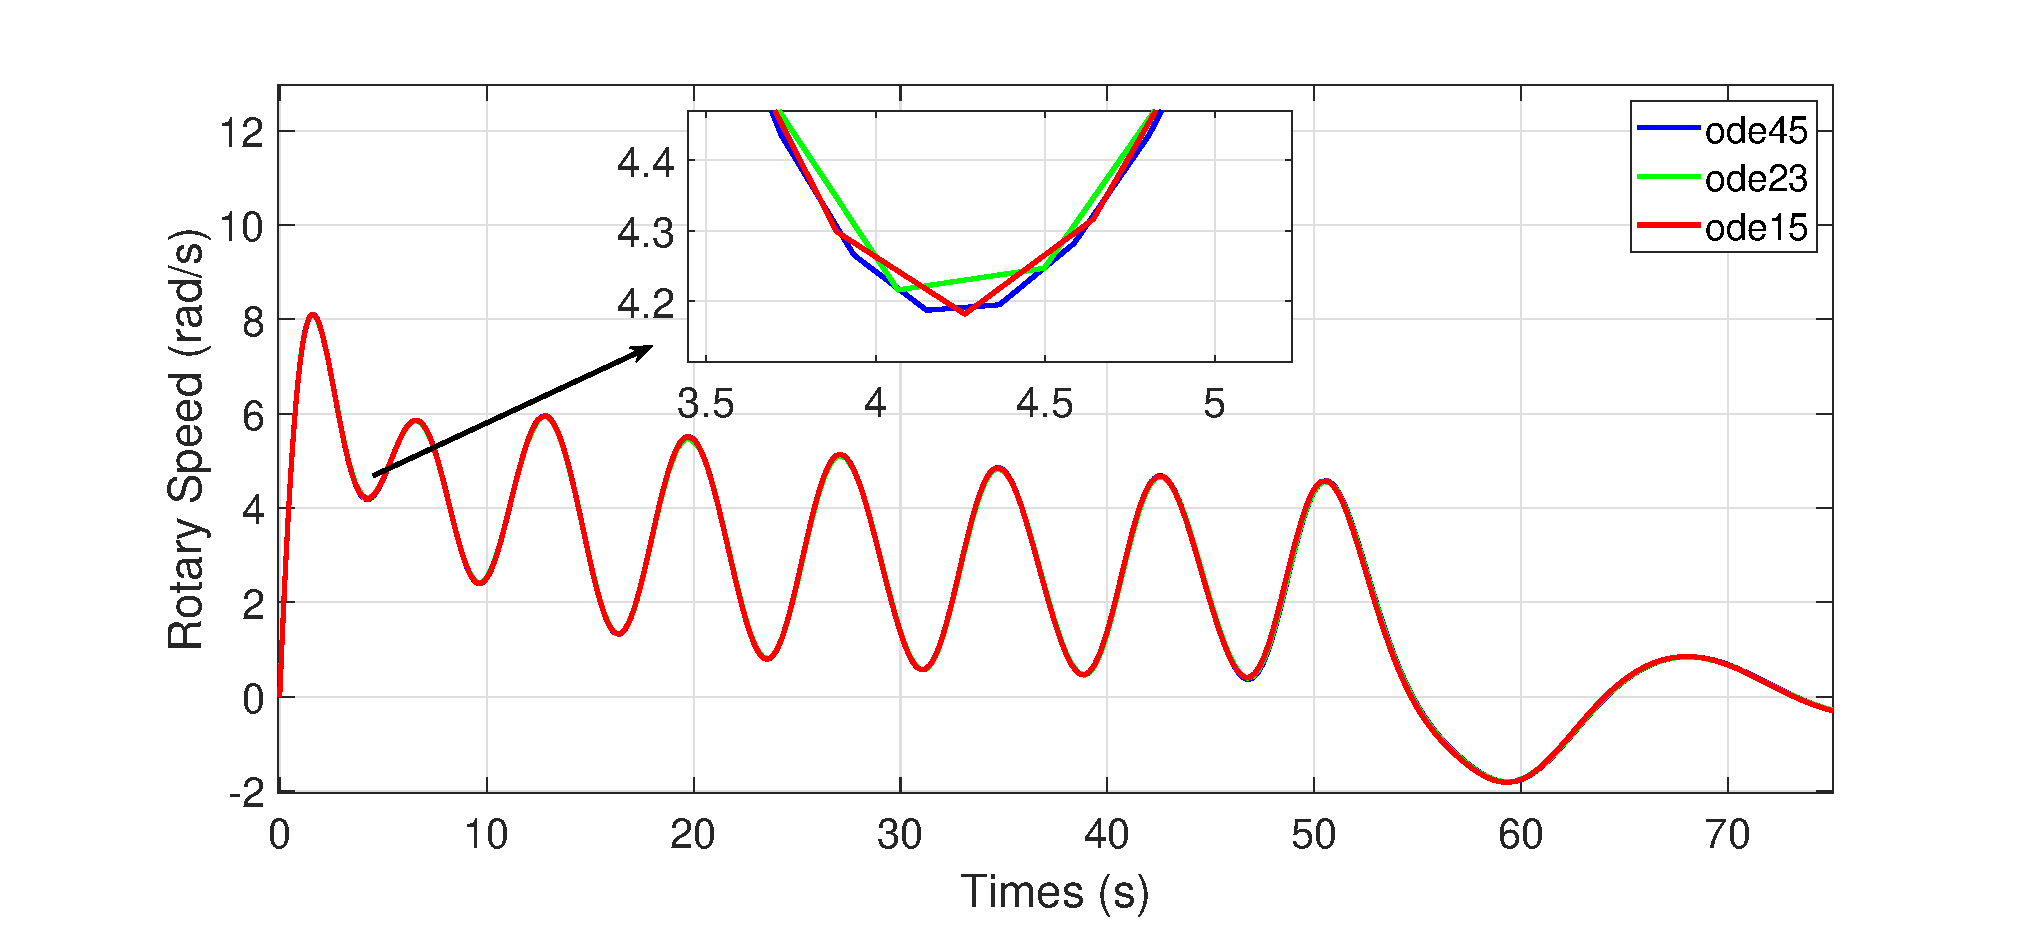
\includegraphics[width=0.8\linewidth]{figures/未加控制三种ode函数求解对比}
		\caption{未加控制三种ode函数求解对比}
		\label{fig:未加控制三种ode函数求解对比}
	\end{figure}
	
	
	可以看出ode45的求解精度要好于其他两种。
	
	\newpage
	\subsection{状态观测器控制的钻柱模型}
	
	状态观测器控制模型:
	
	\begin{figure}[!htbp]
		\centering
		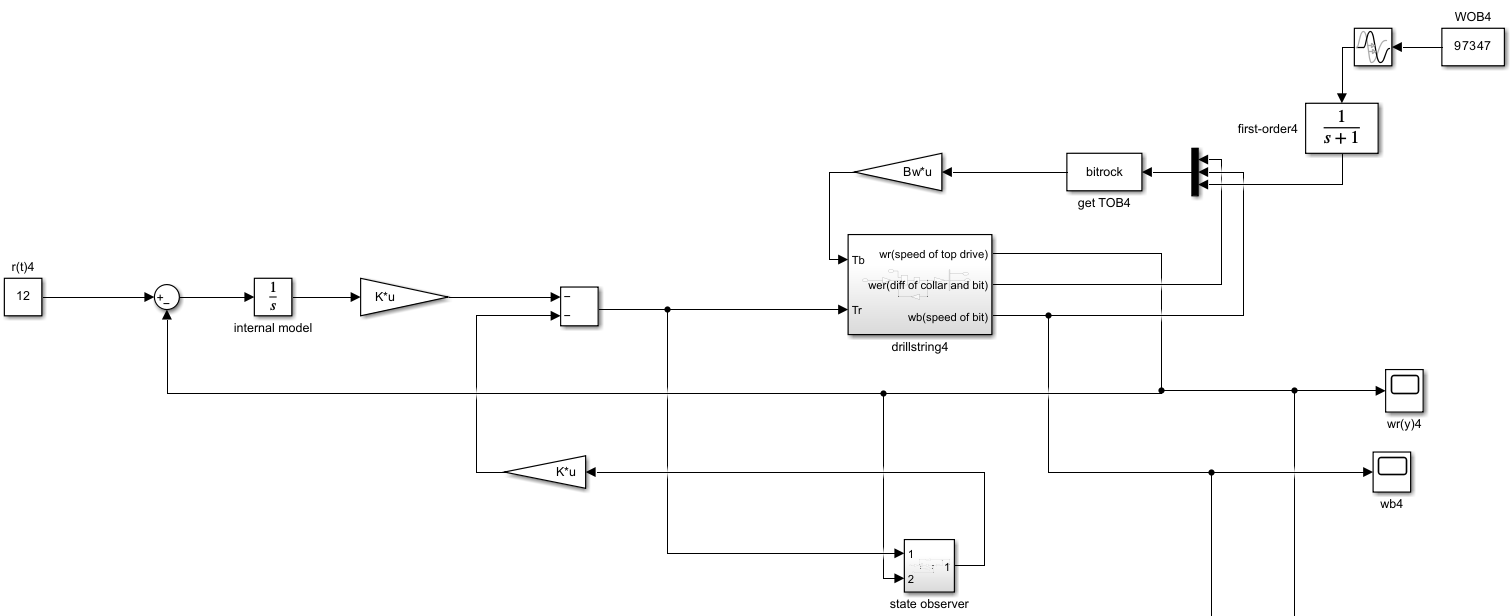
\includegraphics[width=0.7\linewidth]{figures/状态观测器控制}
		\caption{状态观测器控制模型}
		\label{fig:状态观测器控制模型}
	\end{figure}
	
	状态观测器子系统:
	
	\begin{figure}[!htbp]
		\centering
		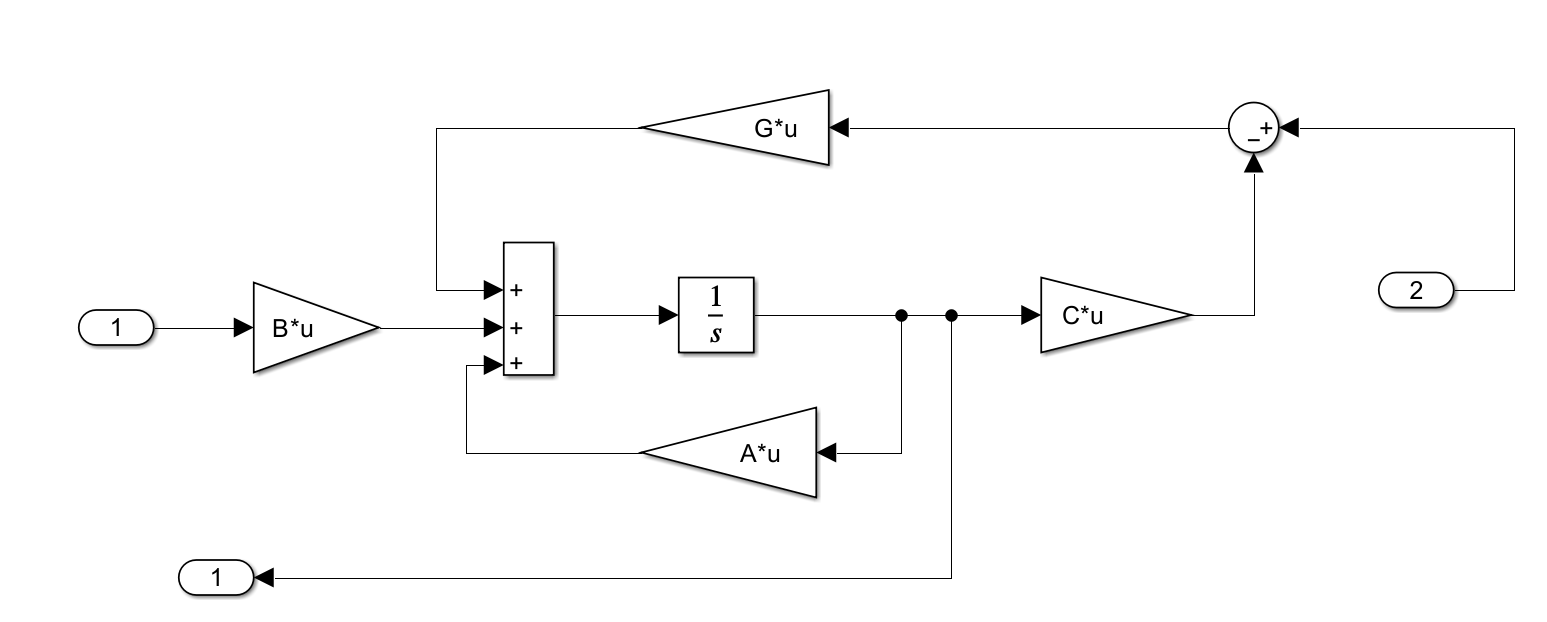
\includegraphics[width=0.7\linewidth]{figures/状态观测器子系统}
		\caption{状态观测器子系统}
		\label{fig:状态观测器子系统}
	\end{figure}
	
	使用LQR方法进行极点配置,权重$Q$和$R$权重:
	
	\begin{equation}
		Q = {\rm{ }}diag\{ 1,{\rm{ }}1,{\rm{ }}1,{\rm{ }}10,{\rm{ }}1,{\rm{ }}1,{\rm{ }}1,{\rm{ }}1000\} ,{\rm{ }}R = {\rm{ }}0.001
	\end{equation}
	
	状态反馈增益和内模增益:
	\begin{equation}
		{K_s}|{K_R} = {\rm{ }}[735.3,{\rm{ }}2490.5,{\rm{ }}504.9,{\rm{ }}247.6611.6,{\rm{ }}909.0,{\rm{ }}959.5|1000]
	\end{equation}
	
	状态观测器增益:
	\begin{equation}
		L = [12.22, 178.38, − 301.66,	−80.86, −52.89, − 580.81, 633.20]^T
	\end{equation}
	
	
	\newpage
	设定预期转速$r=12m/s$,状态观测器对于Bit Speed的观测效果如\autoref{fig:状态观测器控制效果}
	
	\begin{figure}[!htbp]
		\centering
		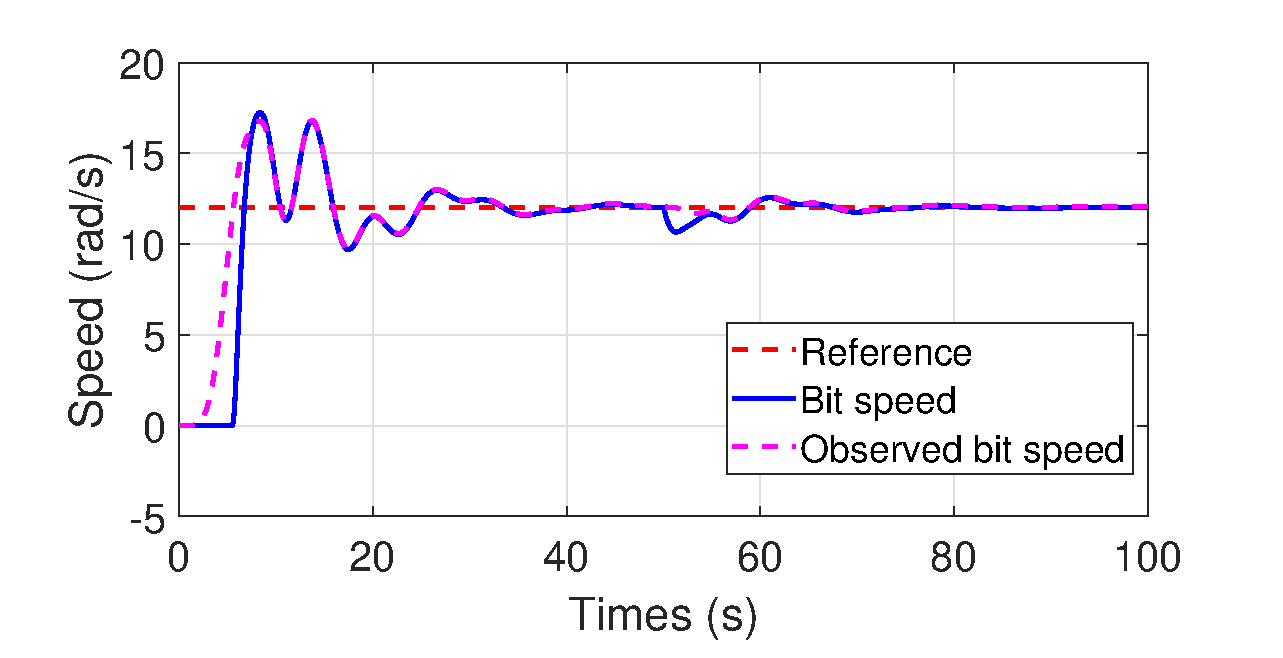
\includegraphics[width=0.7\linewidth]{figures/状态观测器观测效果}
		\caption{状态观测器观测效果}
		\label{fig:状态观测器观测效果}
	\end{figure}
	
	可见状态观测器对于Bit Speed的观测效果很好。
	
	
	状态观测器对于Rotary speed和Bit Speed的控制效果如\autoref{fig:状态观测器观测效果}
	
	\begin{figure}[!htbp]
		\centering
		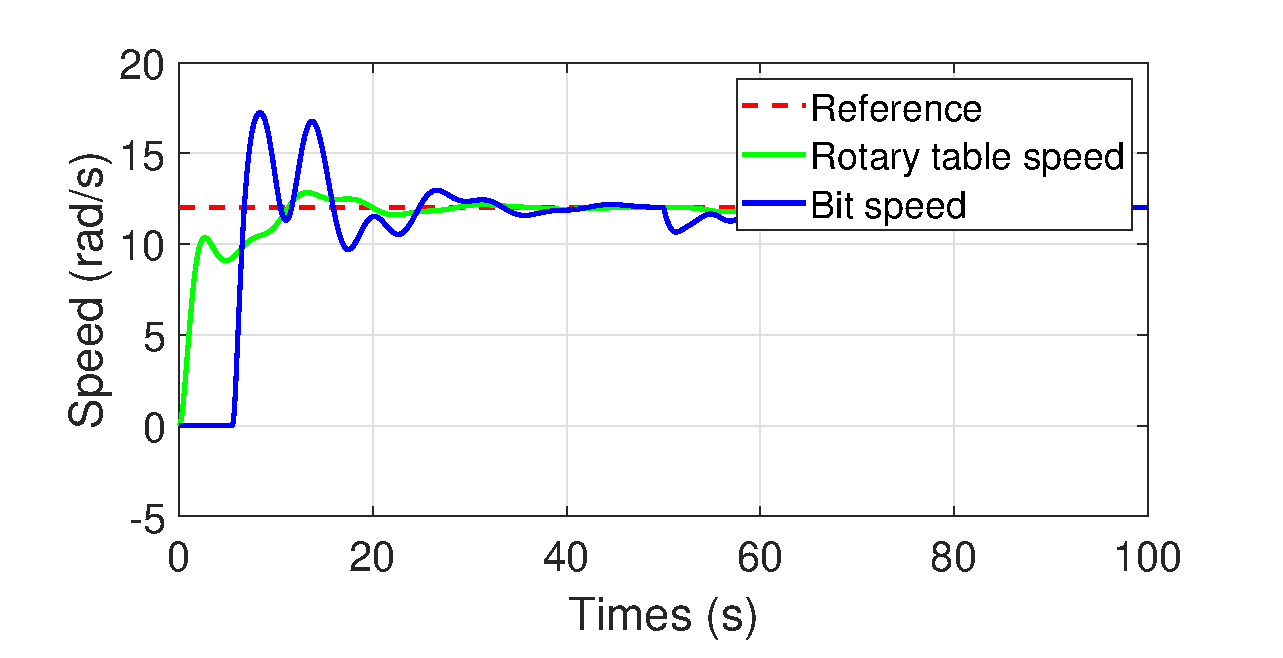
\includegraphics[width=0.7\linewidth]{figures/状态观测器控制效果}
		\caption{状态观测器控制效果}
		\label{fig:状态观测器控制效果}
	\end{figure}
	
	
	可见状态观测器能很快让系统稳定。
	
	\newpage
	
	\subsection{PID控制的钻柱模型}
	
	PID控制模型:
	
	\begin{figure}[!htbp]
		\centering
		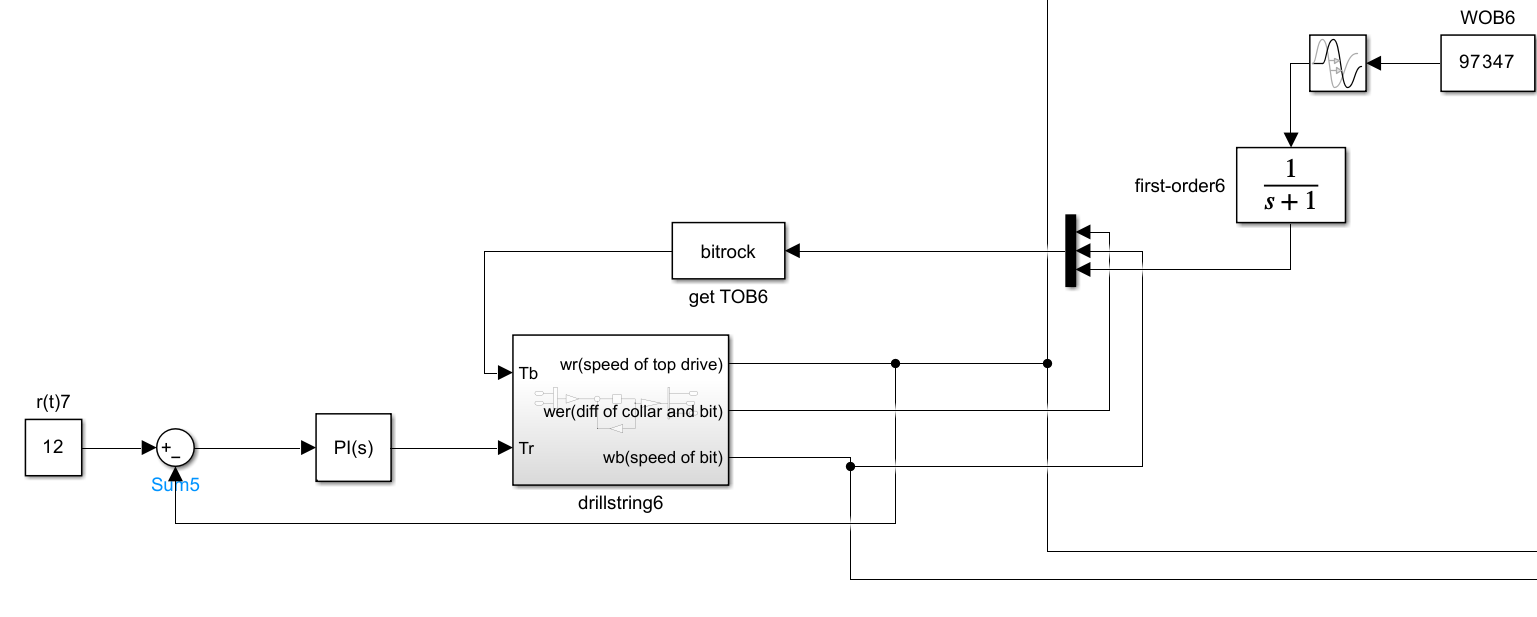
\includegraphics[width=0.7\linewidth]{figures/PID控制模型}
		\caption{PID控制模型}
		\label{fig:PID控制模型}
	\end{figure}
	
	由于扭矩很大,所以P的参数要适当调大一点。
	
	
	PID控制的Rotary Speed:
	
	
	
	PI参数为$P=100,I=0$:
	
	
	
	\begin{figure}[!htbp]
		\centering
		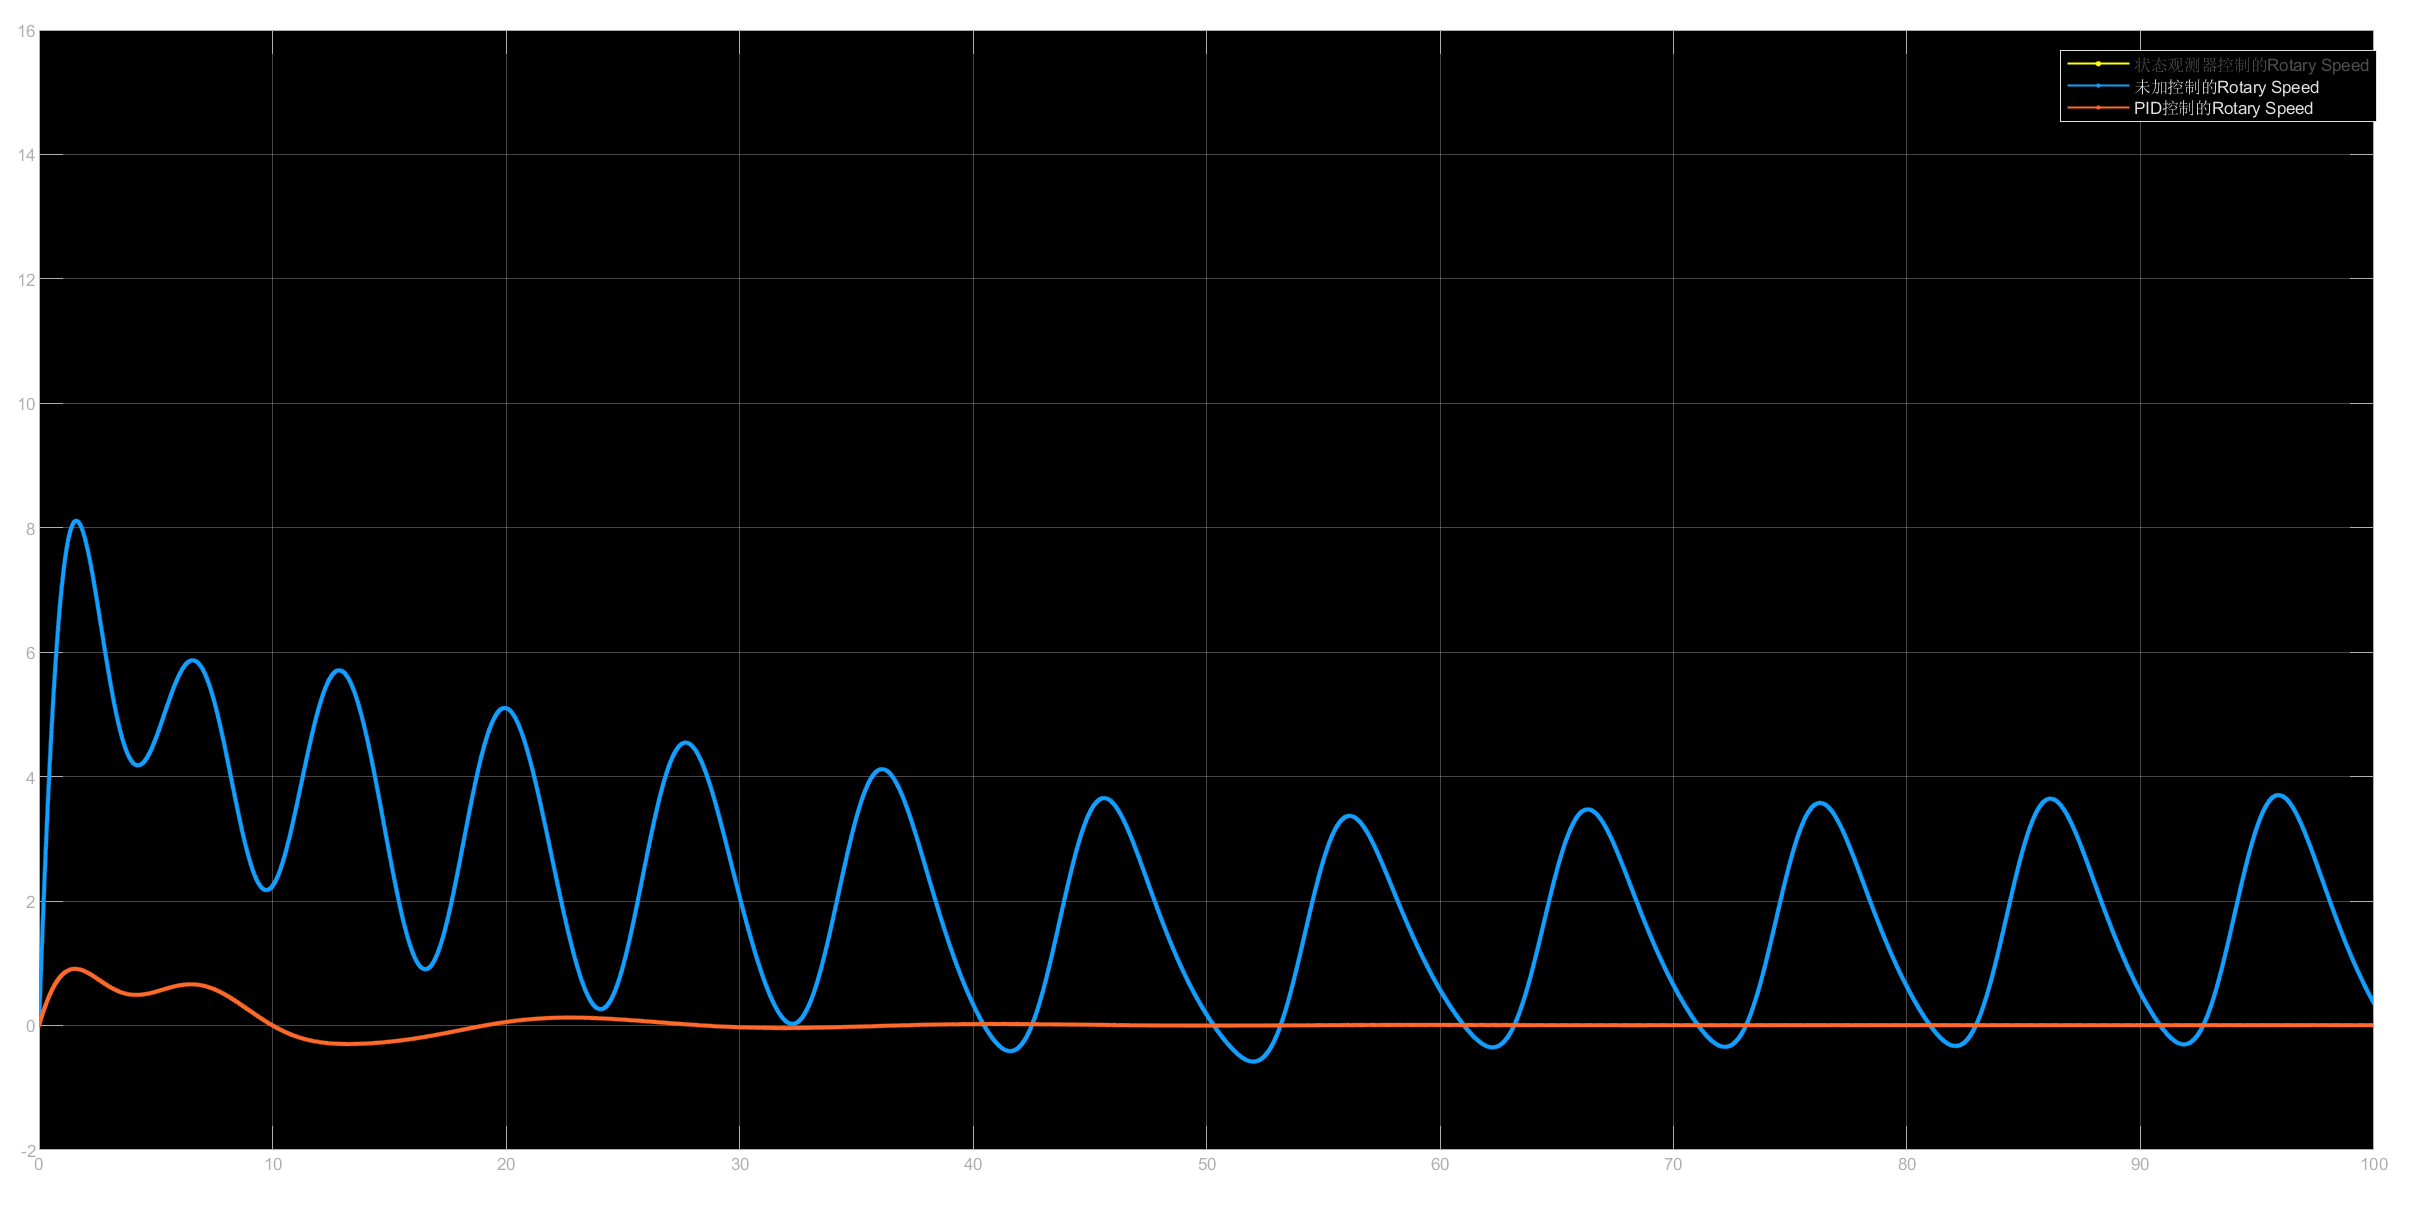
\includegraphics[width=0.7\linewidth]{figures/Rotary_Speed_PID控制_P100}
		\caption{Rotary Speed PID控制 P=100}
		\label{fig:Rotary_Speed_PID控制_P100}
	\end{figure}
	
	
	PI参数为$P=100,I=30$:
	
	\begin{figure}[!htbp]
		\centering
		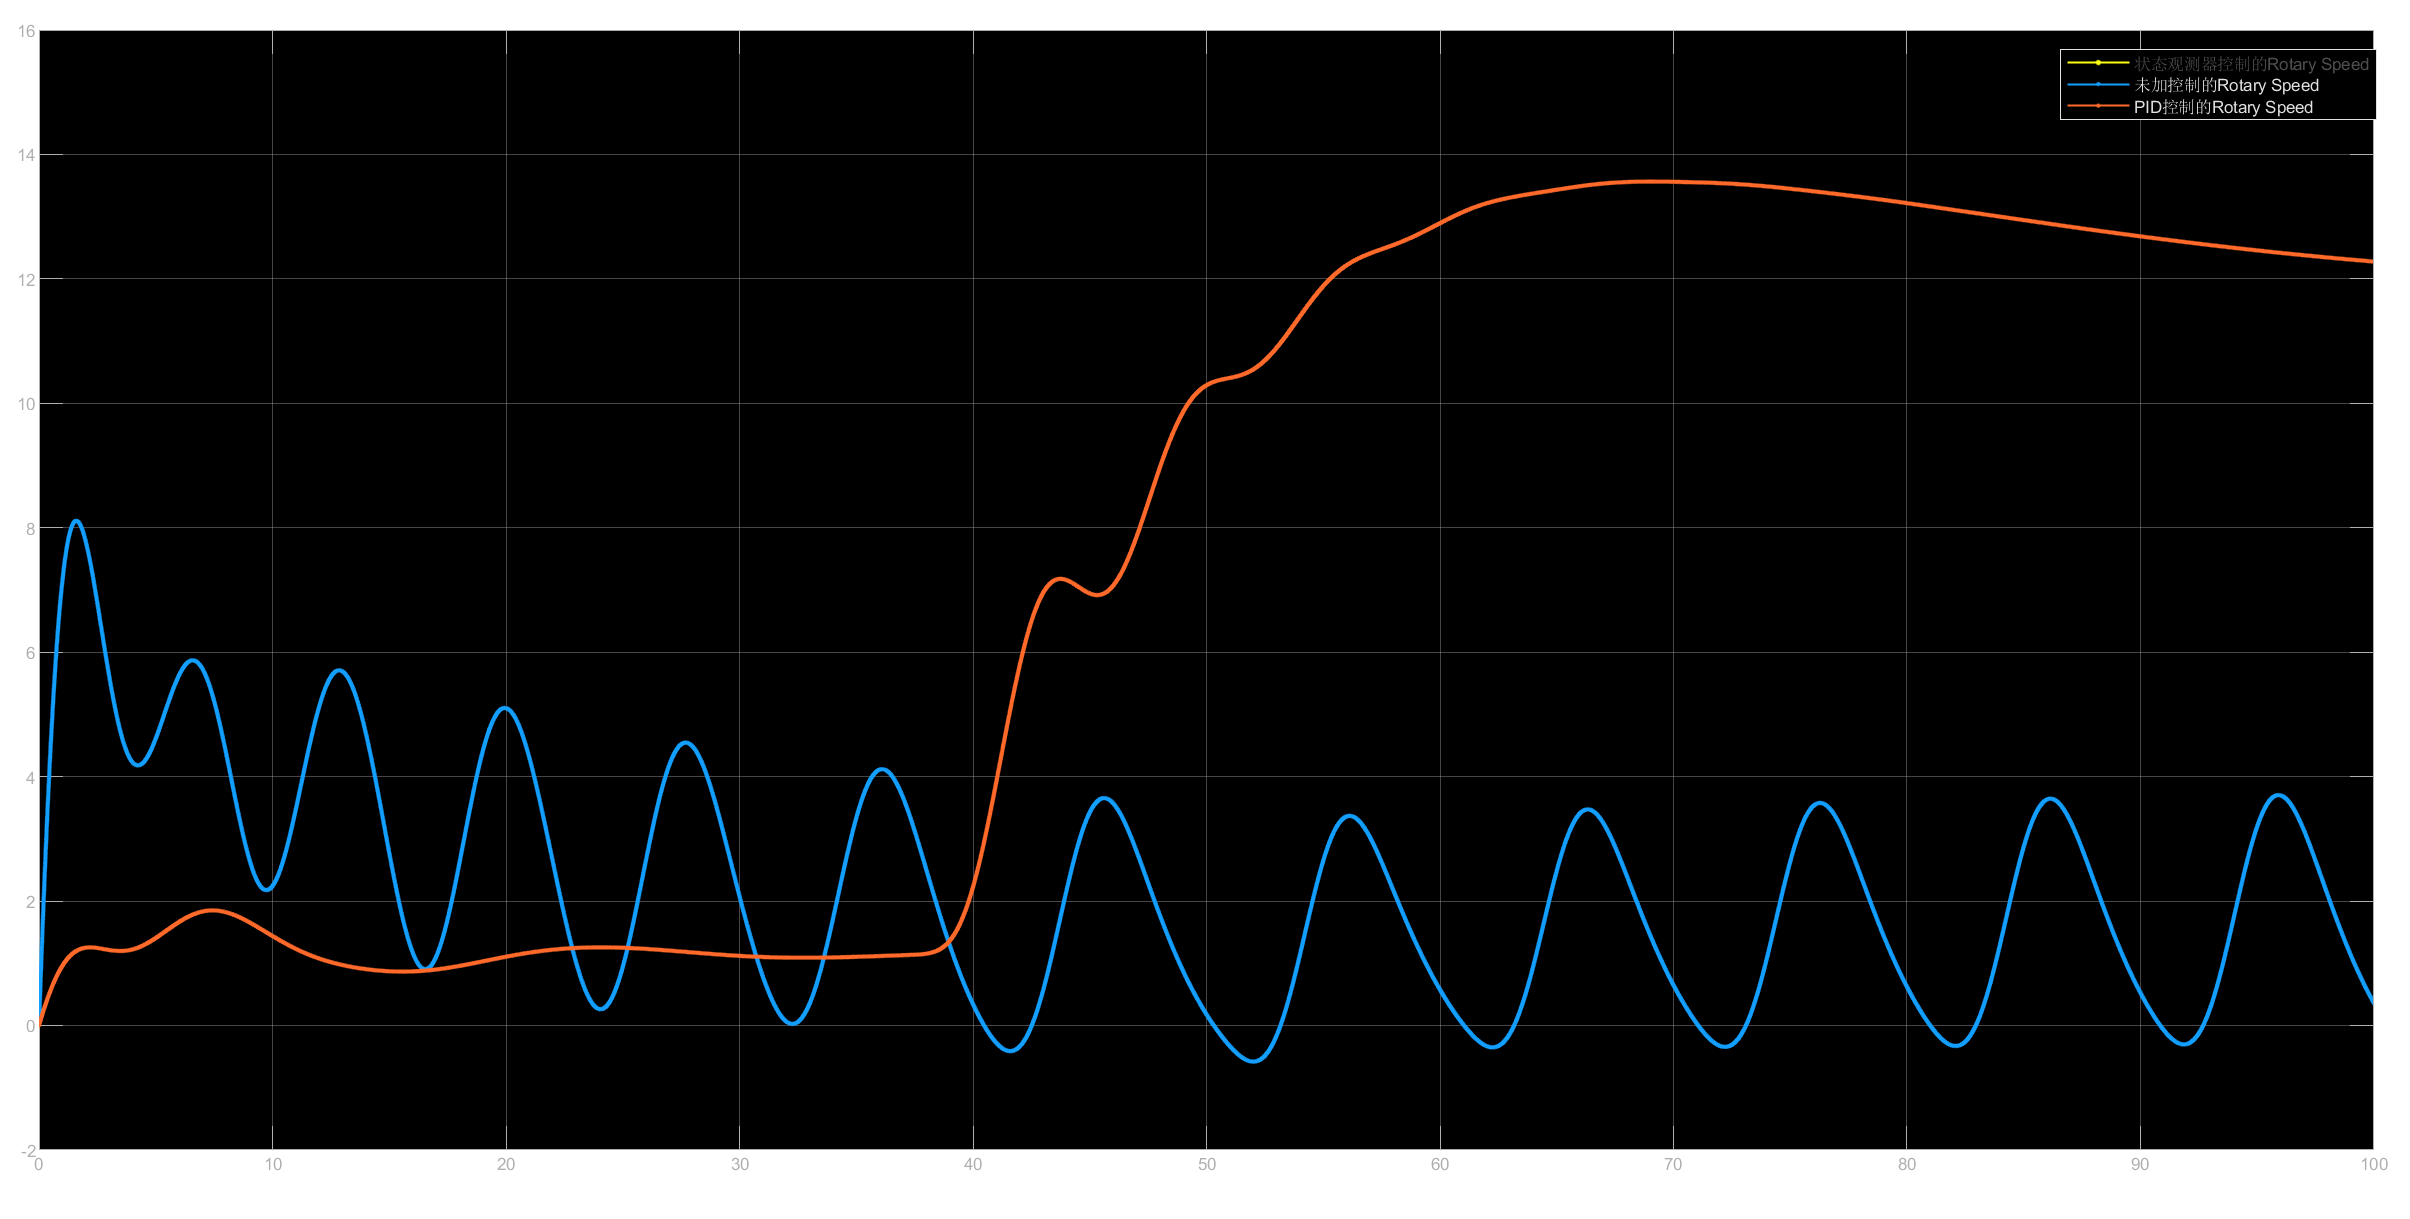
\includegraphics[width=0.7\linewidth]{figures/Rotary_Speed_PID控制_P100_I30}
		\caption{Rotary Speed PID控制 $P=100,I=30$}
		\label{fig:Rotary_Speed_PID控制_P100_I30}
	\end{figure}
	
	
	PI参数为$P=1000,I=100$:
	
	
	
	\begin{figure}[!htbp]
		\centering
		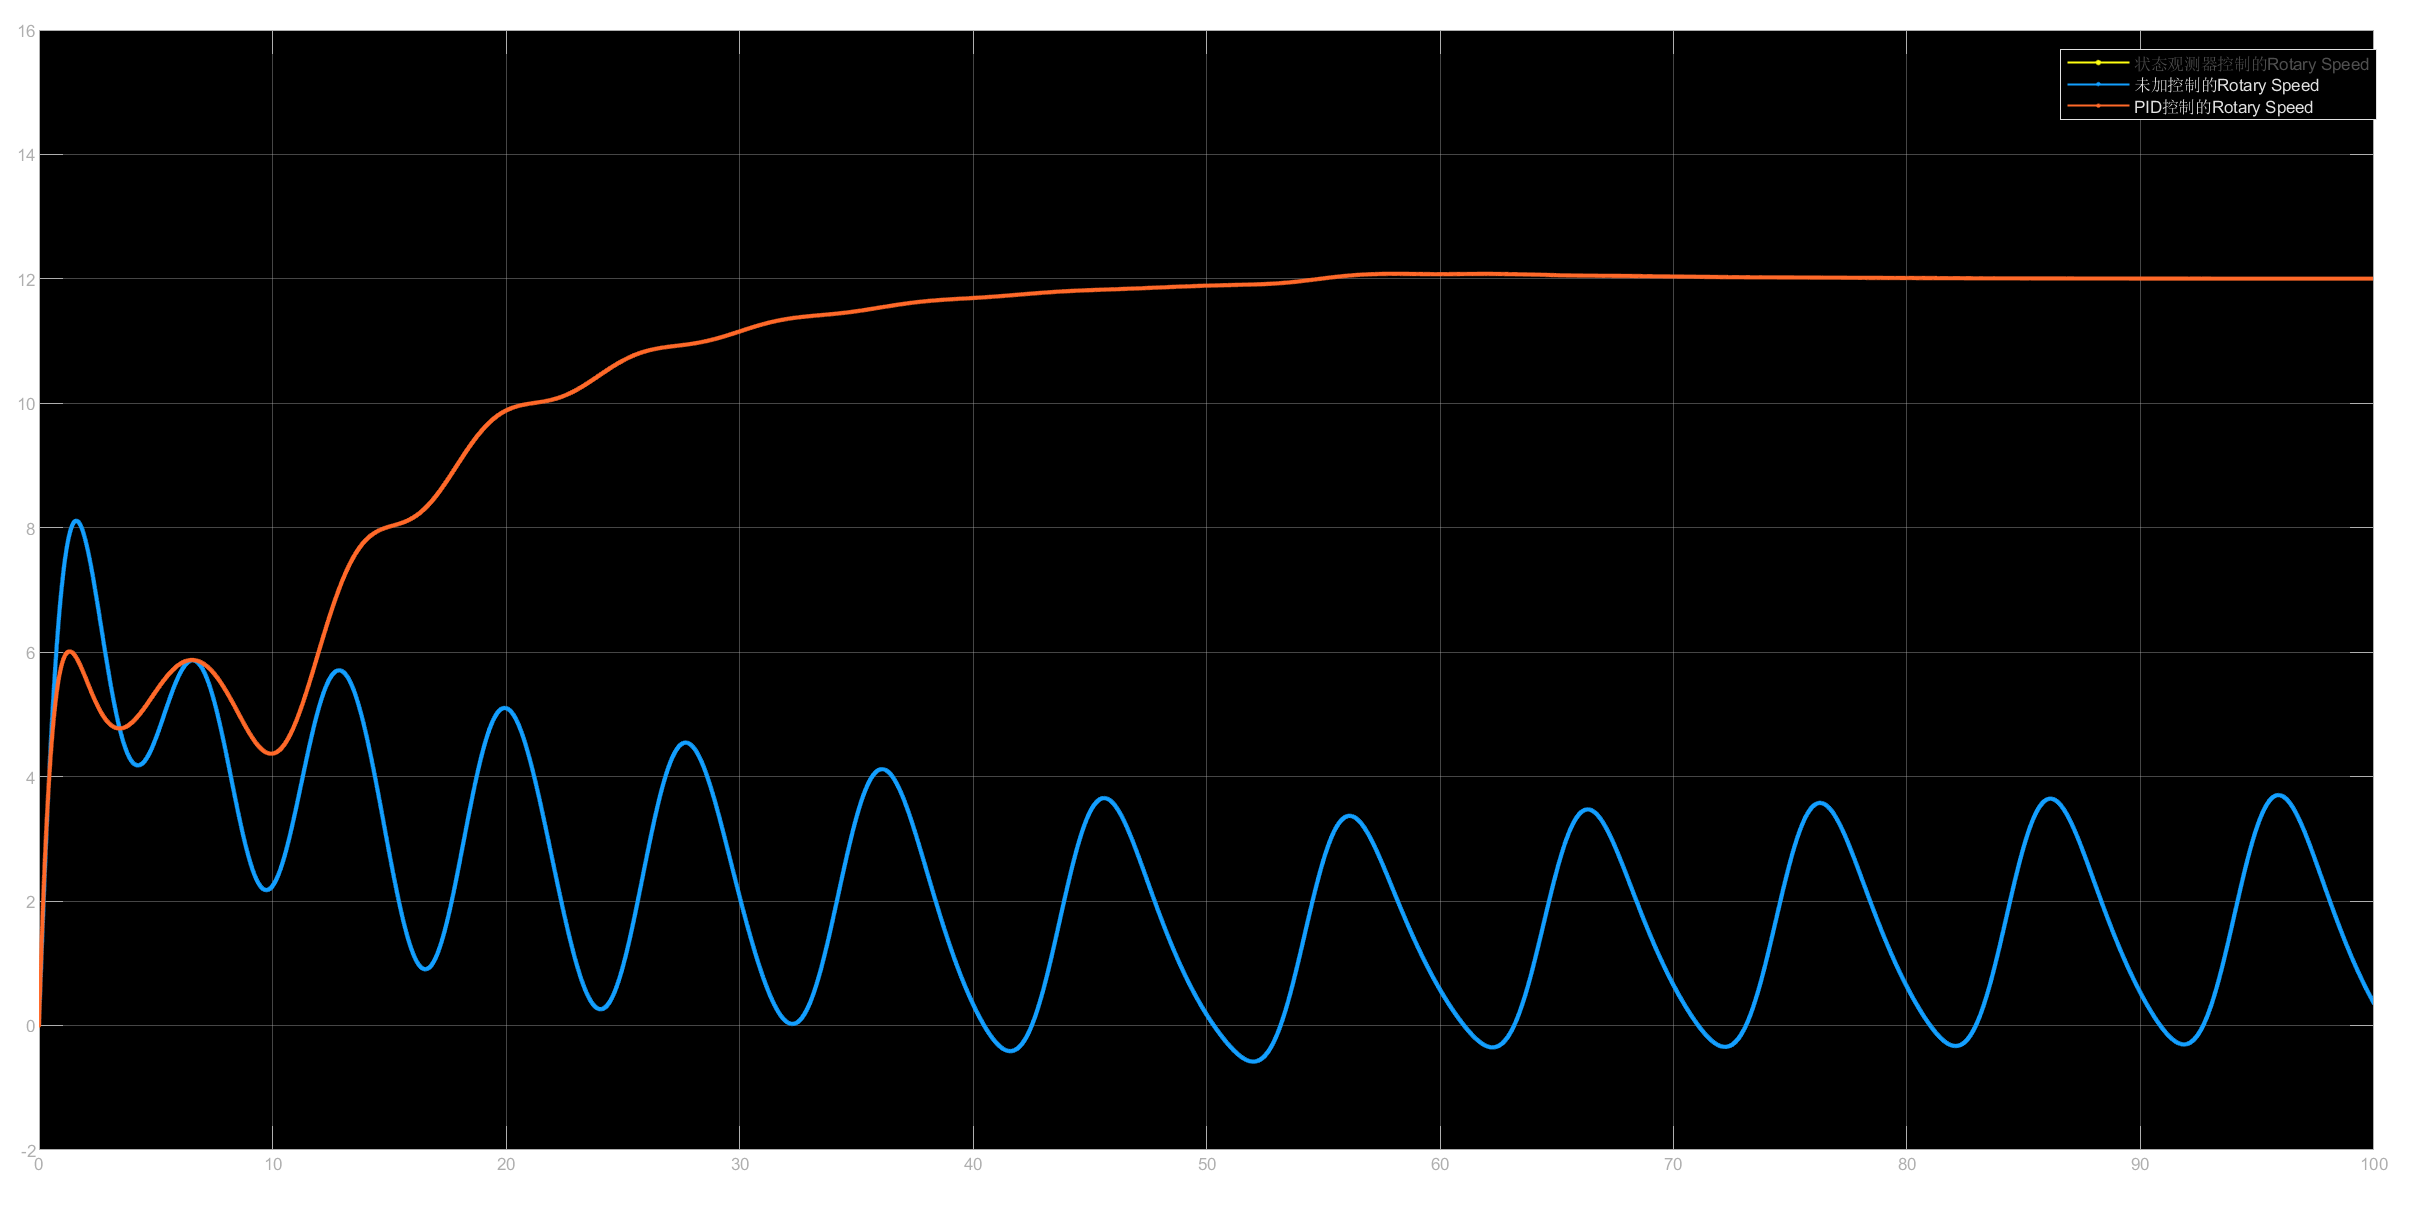
\includegraphics[width=0.7\linewidth]{figures/Rotary_Speed_PID控制_P1000_I100}
		\caption{Rotary Speed PID控制 $P=1000,I=100$}
		\label{fig:Rotary_Speed_PID控制_P1000_I100}
	\end{figure}
	
	
	PI参数为$P=1000,I=300$:
	
	
	
	\begin{figure}[!htbp]
		\centering
		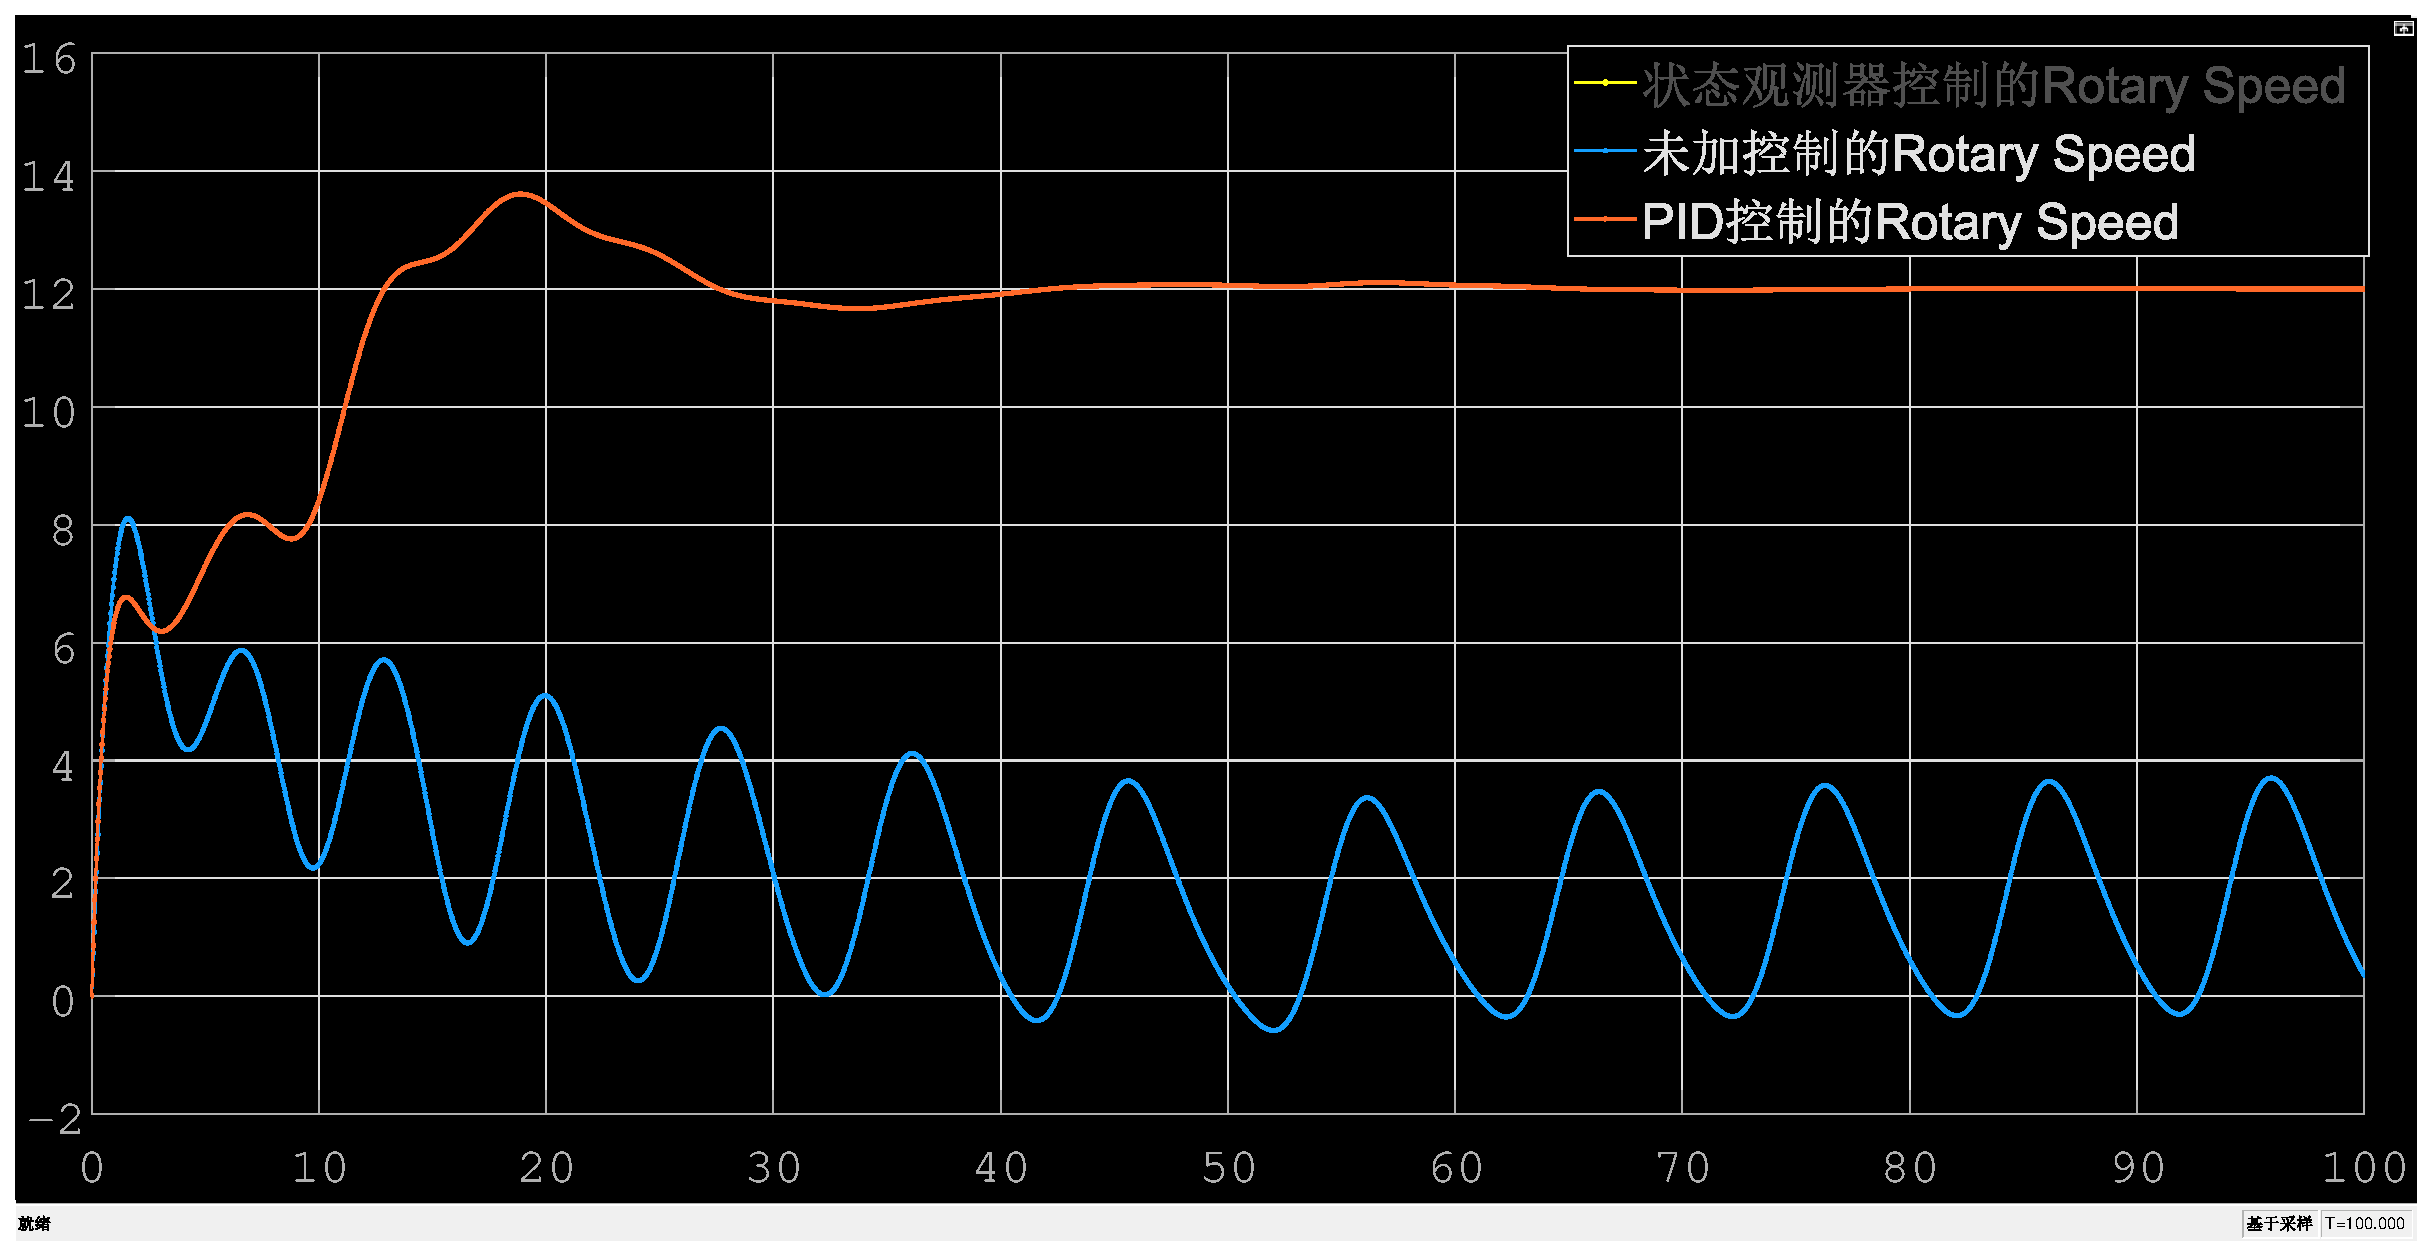
\includegraphics[width=0.7\linewidth]{figures/Rotary_Speed_PID控制}
		\caption{Rotary Speed PID控制 $P=1000,I=300$}
		\label{fig:Rotary_Speed_PID控制}
	\end{figure}
	
	
	
	PI参数为$P=1500,I=300$:
	
	
	
	\begin{figure}[!htbp]
		\centering
		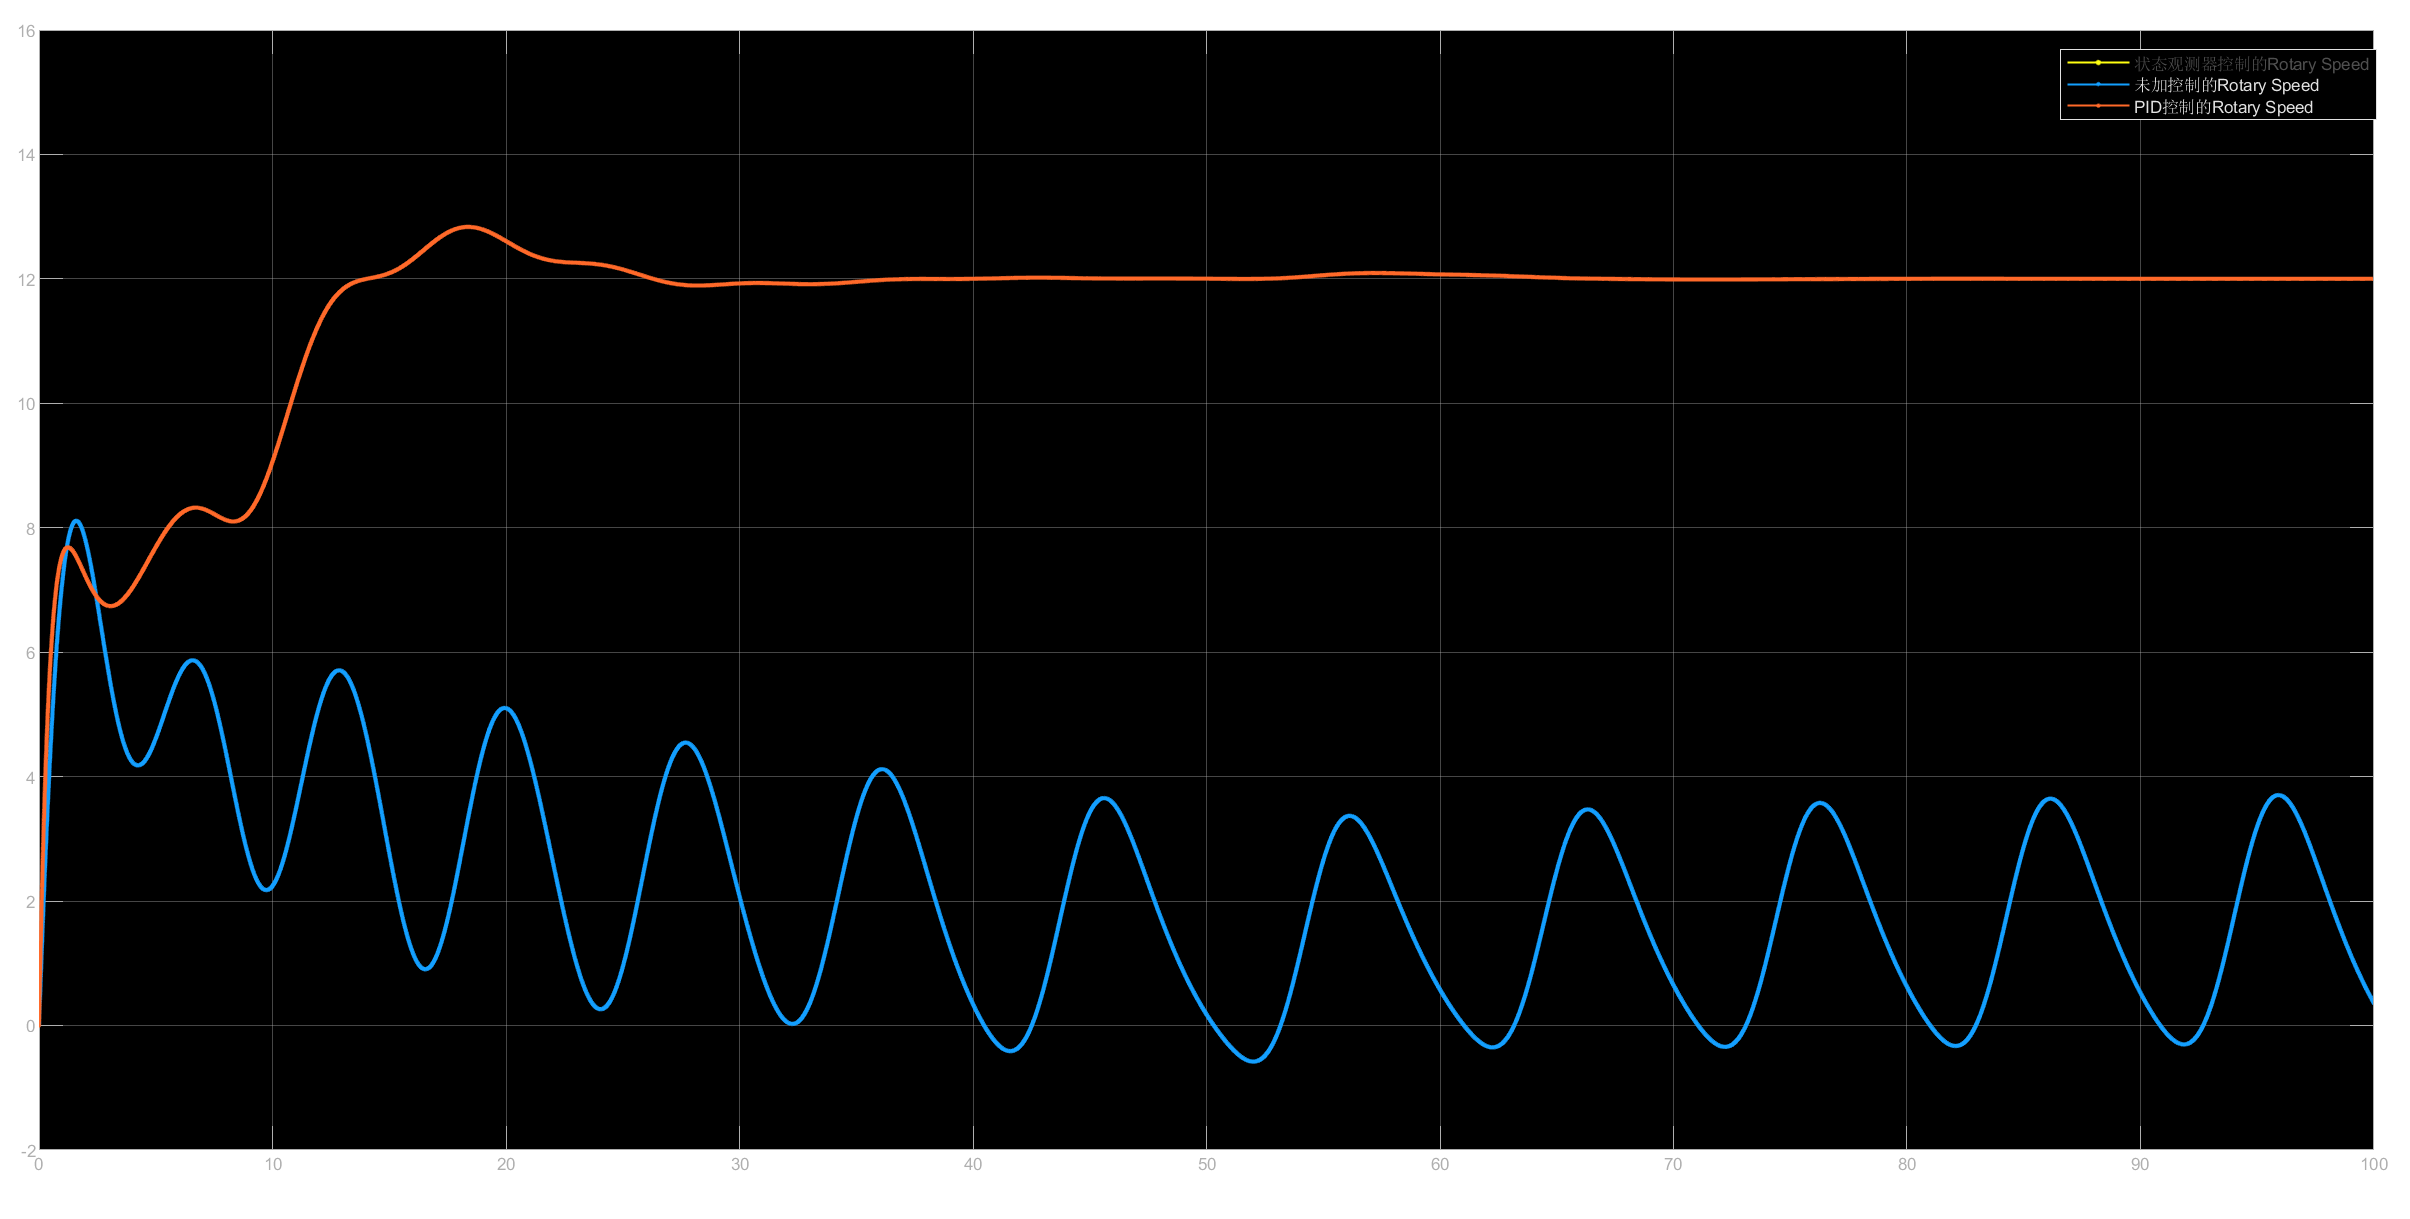
\includegraphics[width=0.7\linewidth]{figures/Rotary_Speed_PID控制_P1500_I300}
		\caption{Rotary Speed PID控制 $P=1500,I=300$}
		\label{fig:Rotary_Speed_PID控制_P1500_I300}
	\end{figure}
	
	可见该参数的控制最好。
	
	\subsection{单神经元PID控制}
	单神经元PID控制是一种结合了经典PID(比例-积分-微分)控制器与神经网络技术的控制方法。其核心思想是利用单个神经元的学习能力来调整PID控制器的参数,以实现对动态系统的自适应控制。
	
	单神经元PID控制Simulink模型:
	\begin{figure}[!htbp]
		\centering
		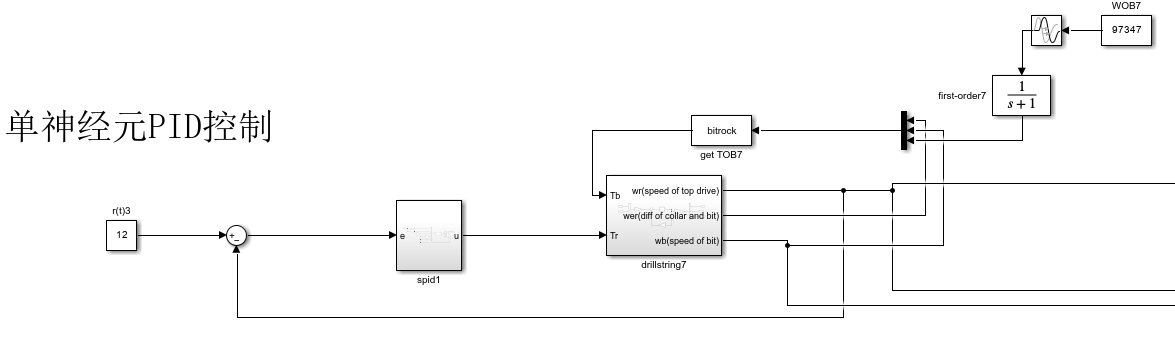
\includegraphics[width=0.7\linewidth]{figures/单神经元PID控制模型.png}
		\caption{单神经元PID控制模型}
		\label{fig:单神经元PID控制模型}
	\end{figure}
	
	\begin{figure}[!htbp]
		\centering
		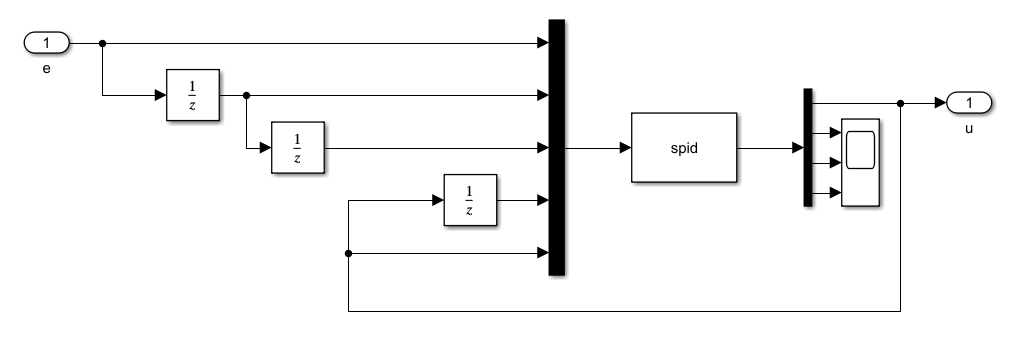
\includegraphics[width=0.7\linewidth]{figures/单神经元PID控制子系统.png}
		\caption{单神经元PID控制子系统}
		\label{fig:单神经元PID控制子系统}
	\end{figure}
	
	控制效果:
	
	\begin{figure}[!htbp]
		\centering
		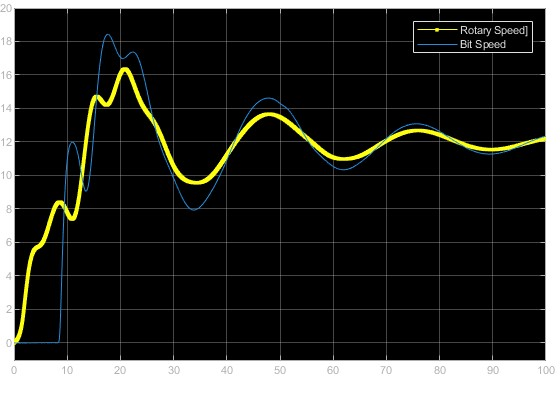
\includegraphics[width=0.7\linewidth]{figures/spid控制效果}
		\caption{spid控制效果}
		\label{fig:spid控制效果}
	\end{figure}
	
	由于控制效果不佳,所以接下来不与前两种控制方法进行对比。
	
	\subsection{控制效果对比}
	
	下面进行状态观测器和PID的控制效果对比。
	
	Rotary Speed控制对比:
	
	
	\begin{figure}[!htbp]
		\centering
		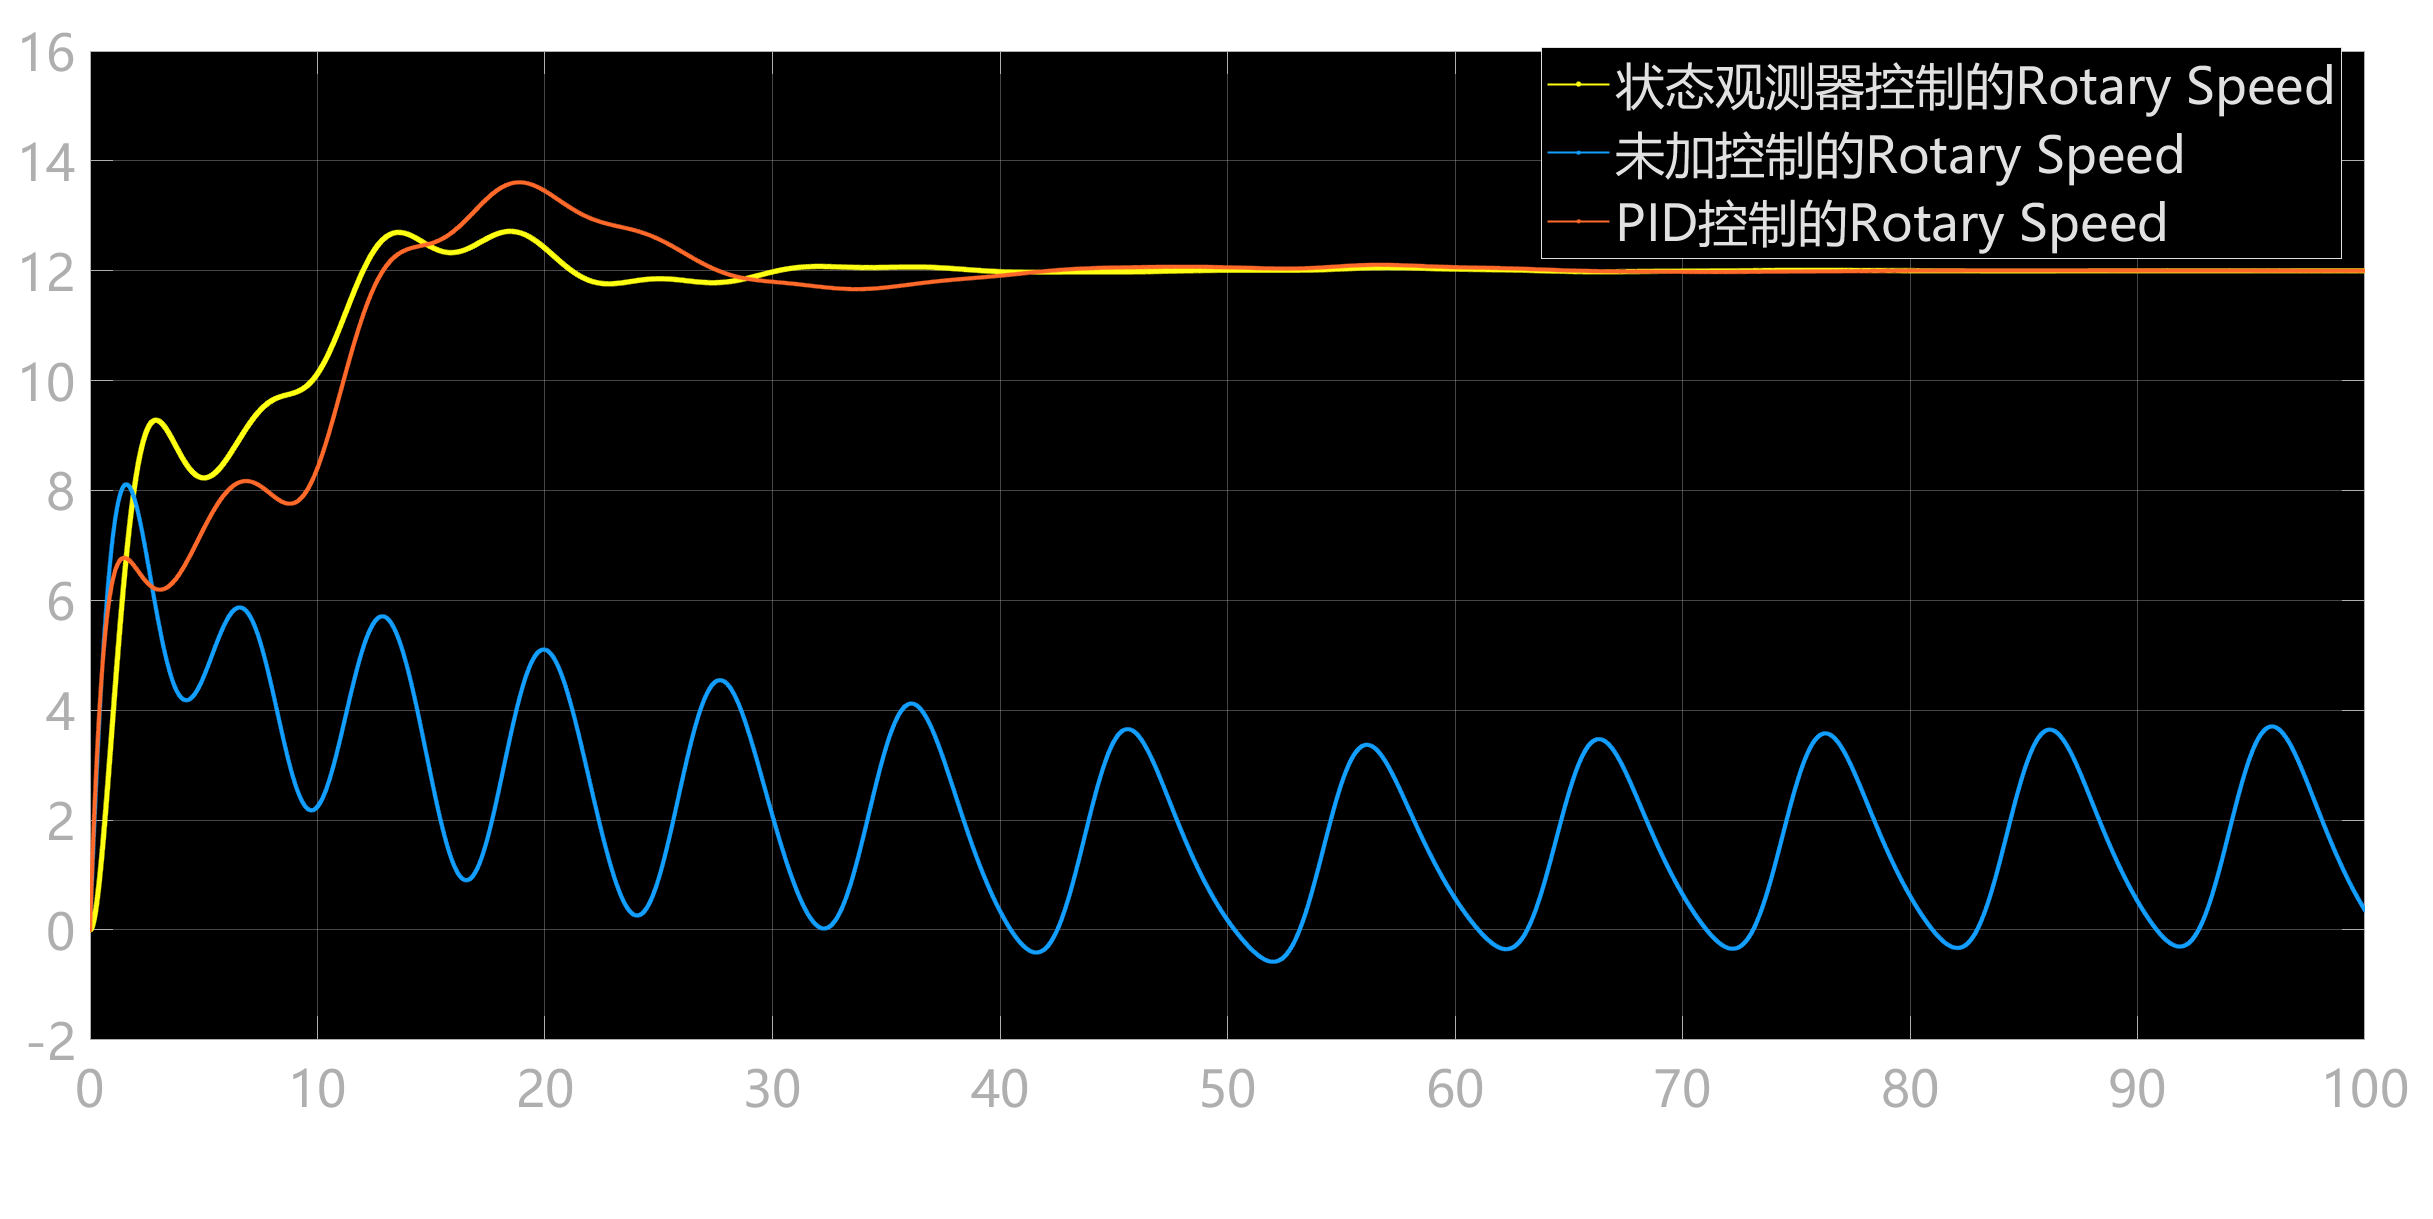
\includegraphics[width=0.7\linewidth]{figures/Rotary_Speed控制对比}
		\caption{Rotary Speed控制对比}
		\label{fig:Rotary_Speed控制对比}
	\end{figure}
	
	
	Bit Speed控制对比:
	
	\begin{figure}[!htbp]
		\centering
		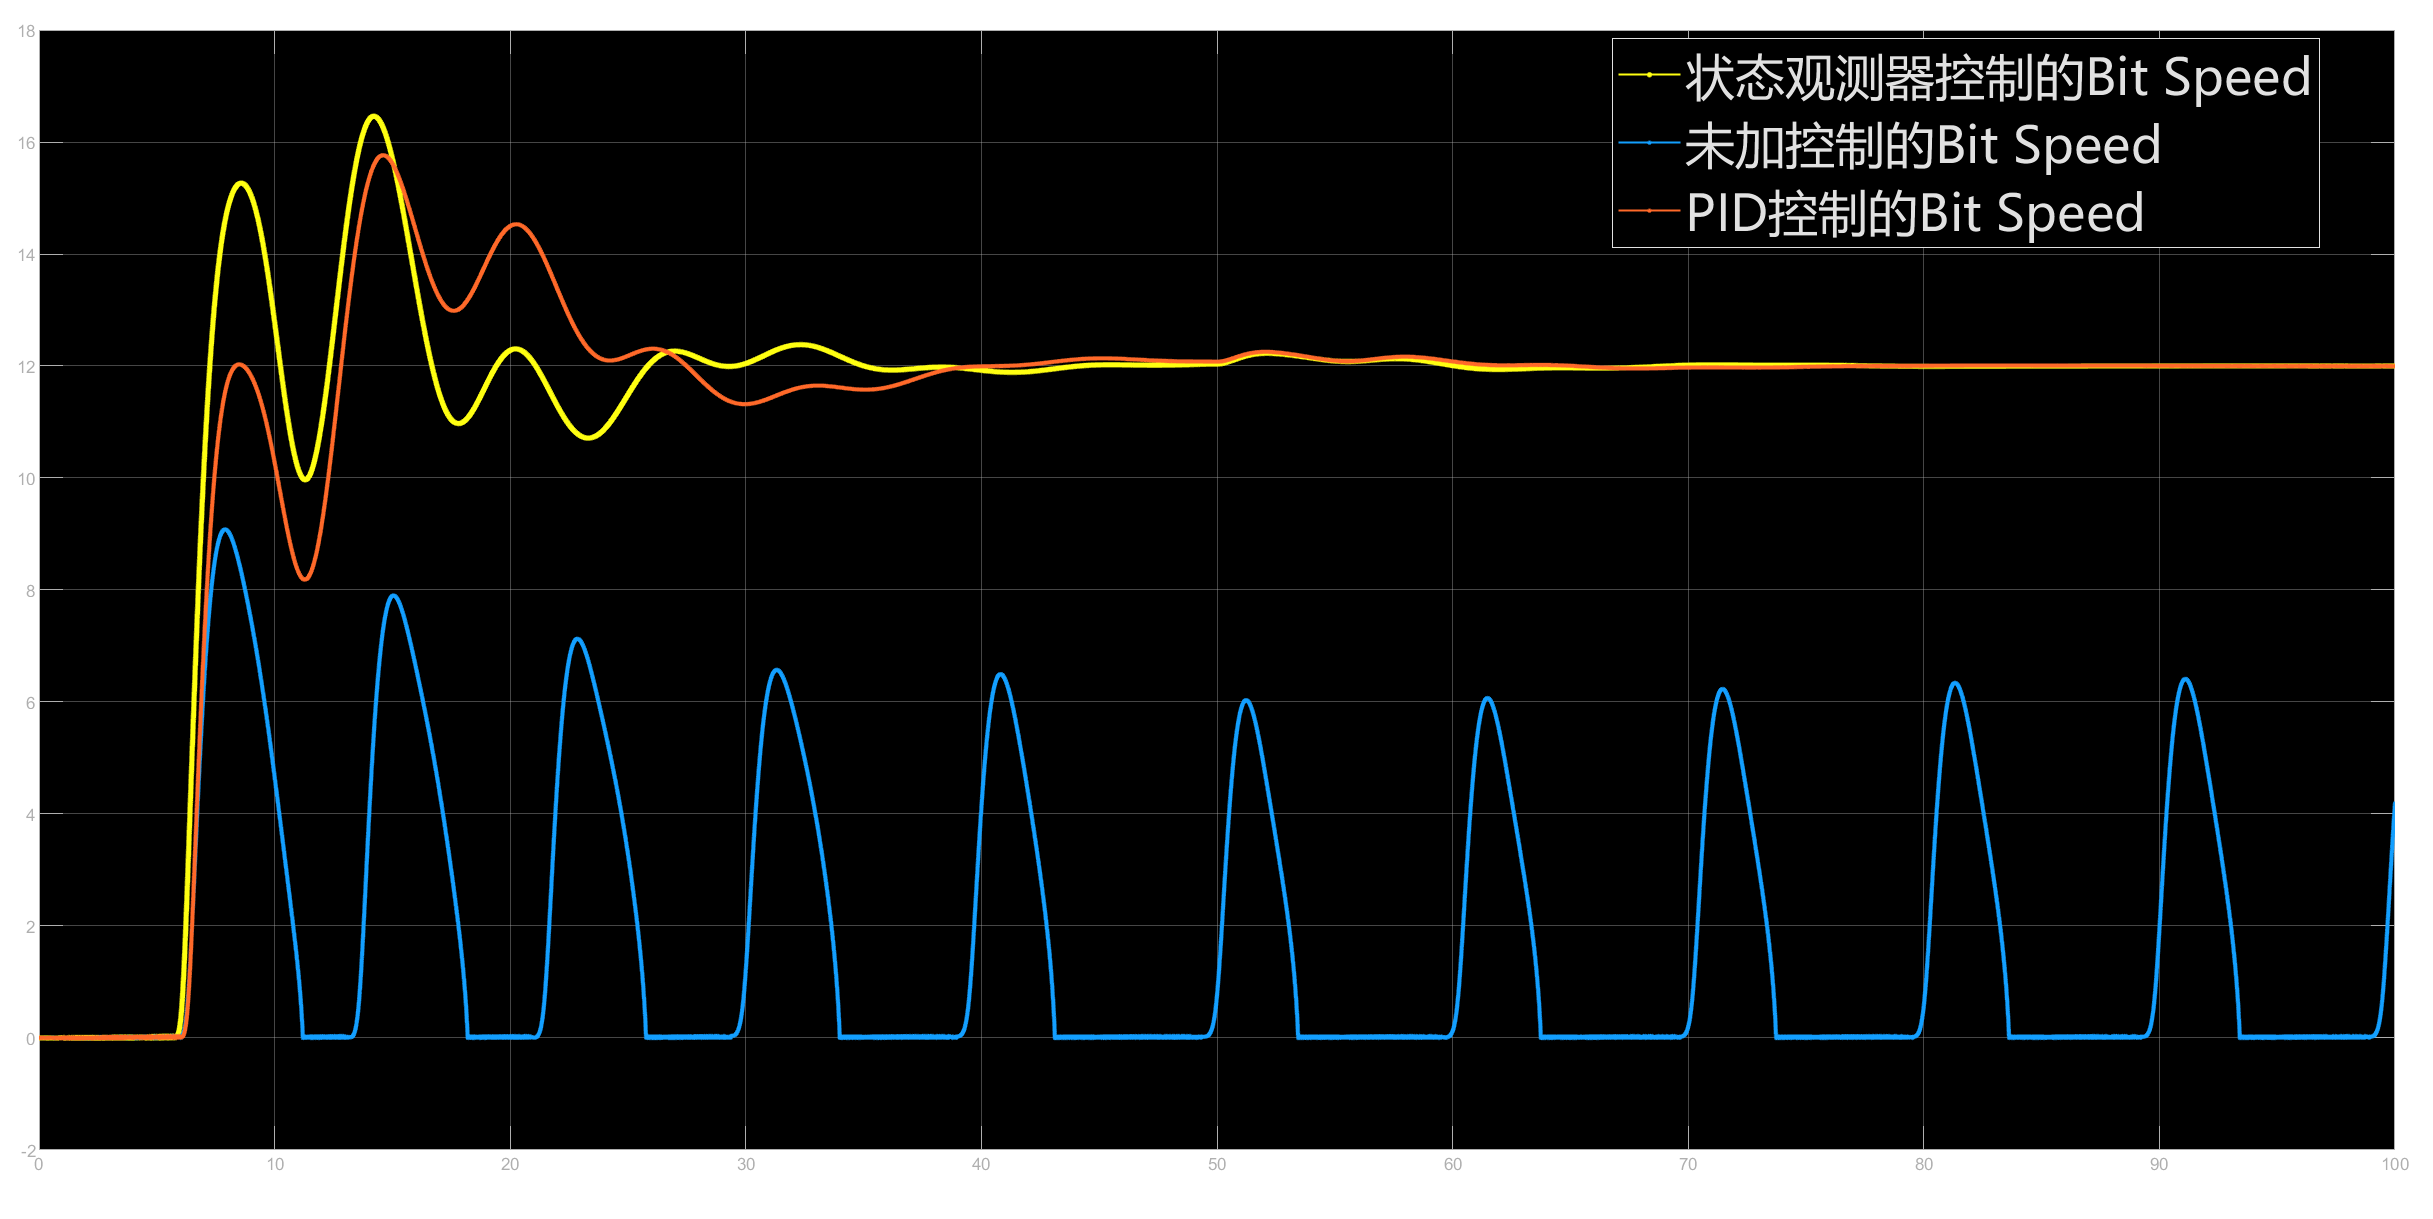
\includegraphics[width=0.7\linewidth]{figures/Bit_Speed控制对比}
		\caption{Bit Speed控制对比}
		\label{fig:Bit_Speed控制对比}
	\end{figure}
	
	可见状态观测器的控制效果比PID控制要好
	
	
	\newpage
	\section{总结}
	
	钻井作业过程中存在着横向振动,轴向振动和扭转振动等多种振动形式,而钻柱粘滑振动属于钻柱的扭转振动,并且是影响钻井作业最严重的振动现象。由于钻柱粘滑振 动的产生,使得钻井设备过早损坏,钻井完井周期变长,钻井作业安全性下降和钻井效率降低等诸多不利影响。钻柱粘滑振动的产生是由钻头与井下岩石切削产生的摩擦力矩 和顶部驱动系统传递到钻头的驱动扭矩之间的大小关系决定,钻柱的粘滑振动使得钻头 在一段时间粘滞不动,过一段时间又以超高速转动,如此往复循环,对钻井作业产生极 大的影响。本文为了抑制钻柱粘滑振动现象,分析了钻柱系统粘滑振动的产生原因,建立了系统力学模型及仿真模型,并设计了状态观测器反馈控制和PID控制来抑制钻柱粘滑振动的产生。具体的研究内容总结如下:
	
	
	
	(1)钻柱粘滑振动的机理分析。
	
	对钻柱系统的组成及各部分的工作原理进行了解, 在了解钻柱系统组成之后,结合钻井作业流程分析钻柱粘滑振动的产生机理,得到钻柱 粘滑振动现象的产生是由于井下钻头与井底岩石之间的摩擦力矩大于转盘驱动系统通过 钻杆传递到钻头上的驱动扭矩,使得钻头粘滞在岩石上静止不转,当积聚在钻头上的驱 动扭矩远远大于钻头岩石产生的摩擦力矩时,钻头又以超高速反向旋转,此时为滑动状 态,由于钻头是反向旋转,之后转速又会变为零静止在岩石上,又变回粘滞状态,如此 往复,造成粘滞,滑动,粘滞,滑动的往复过程。
	
	(2)钻柱系统的建模。
	
	为了对钻柱系统进行更加详细的分析,将钻柱系统简化为转 盘、钻杆、BHA 和钻头的四自由度扭转模型。模型考虑了钻柱的扭转自由度,钻柱阻尼 和钻头岩石相互作用的高度非线性摩擦,建立了转盘、钻杆、BHA 及钻头四部分简化模 型的运动微分方程,通过运动微分方程得出系统的状态空间方程,为下一步进行钻柱系 统仿真实验做准备。
	
	(3) 粘滑振动现象仿真与分析
	
	使用 MATLAB/Simulink 完成钻柱粘滑振动的仿真,仿真结果接近于实际钻进过程钻柱行为,验证了该模型的有效性;分析了钻进过程参数如钻压、参考转速和钻井液阻尼等对钻柱的影响,揭示了钻头-岩石的非线性作用率是造成粘滑振动的根本原因;同时考虑到了钻柱长度对钻柱振动的影响,即随着钻柱的不断加长,降低了钻柱等效的扭转刚度,使得粘滑振动易于发生。
	
	(4) 抑制控制
	
	使用状态观测器反馈控制和PID 的控制策略,在进行控制器模型建立和参数设计后,通过仿真验证了控制策略的有效性,粘滑振动现象被消除,底部钻头转速可以稳定的跟踪顶部输入。
	
	
	
	
	
	
	
	%\section{定理环境}
	%\begin{Theorem}
	%\end{Theorem}
	%
	%\begin{Lemma}
	%\end{Lemma}
	%
	%\begin{Corollary}
	%\end{Corollary}
	%
	%\begin{Proposition}
	%\end{Proposition}
	%
	%\begin{Definition}
	%\end{Definition}
	%
	%\begin{Example}
	%\end{Example}
	%
	%\begin{proof}
	%\end{proof}
	
	
	
	
	
	
	
	%%----------- 参考文献 -------------------%%
	%在reference.bib文件中填写参考文献,此处自动生成
	
	\newpage
	\bibliographystyle{gbt7714-numerical}  % 引用格式
	\bibliography{reference.bib}  % bib源
	
	
	\newpage
	\begin{appendices}
		
		\section{文件列表}
		
		\begin{table}[h]  
			\centering  
			\caption{文件列表}  
			\renewcommand{\arraystretch}{1.25} % 增加行间距  
			\begin{tabular}{c@{\hspace{20pt}}c} % 增加列间距   
				\toprule  
				文件名   & 功能描述 \\
				\midrule  
				main.m & 主程序代码 \\
				drillstring.m & 钻柱模型代码 \\
				LQRPolePlacement.m & LQR极点配置代码 \\
				\toprule  
			\end{tabular}  
			\label{tab:文件列表}  
		\end{table}  
		
		\section{代码}
		\noindent main.m
		\lstinputlisting[language=matlab]{code/main.m}
		drillstring.m
		\lstinputlisting[language=matlab]{code/drillstring.m}
		LQRPolePlacement.m
		\lstinputlisting[language=matlab]{code/LQRPolePlacement.m}
	\end{appendices}
	
	
\end{document}